

\documentclass[]{report}   % list options between brackets


% Latex Police and file encoding
\usepackage[utf8]{inputenc}
\usepackage[T1]{fontenc}  % for character encoding 
\usepackage{lmodern}  % Police setting
\usepackage[american]{babel}


%style of tex :
\setlength{\parskip}{1ex plus 0.5ex minus 0.2ex} %space between paragraphs


% Code Formating
% For code snippets style definition

\usepackage{color}
\usepackage{listings}


\lstloadlanguages{[ISO]C++,C,bash}
% set up listing environment with C syntax hightlight
\definecolor{stringcolor}{rgb}{0.20,0.50,0.20}
\definecolor{commentcolor}{rgb}{0.40,0.40,0.40}
\definecolor{keywordcolor}{rgb}{0.50,0.10,0.10}
\definecolor{idcolor}{rgb}{0.10,0.10,0.50}
\definecolor{bg}{rgb}{0.95,0.95,0.95}
% with \lstset one can predefine parameters for listings
\lstset{language=[ISO]C++,basicstyle=\small,keywordstyle=\color{keywordcolor},
        commentstyle={\color{commentcolor}\itshape},
        stringstyle={\color{stringcolor}},
        identifierstyle=\color{idcolor},numbers=left,
       % xleftmargin=2em,framerule=0.8pt,
        stepnumber=1,
        frame=single,
        showstringspaces=false,
        firstnumber=1,
        numberstyle=\ttfamily,backgroundcolor=\color{bg},
        basicstyle=\ttfamily\footnotesize}
        
        
% Definition of \C++ to be eye candy :
\usepackage{relsize}
\usepackage{lipsum}
%c from texinfo.tex
\def\ifmonospace{\ifdim\fontdimen3\font=0pt }
\def\C++{%
\ifmonospace%
    C++%
\else%
    C\kern-.1667em\raise.30ex\hbox{\smaller{++}}%
\fi%
\spacefactor1000 }

%Inliine listings :
\usepackage{paralist}

%figures :
\usepackage{graphicx}
\usepackage{float}
% wrapped
\usepackage{wrapfig}
%\floatstyle{boxed} 
\restylefloat{figure}

%\usepackage[format=plain,indention=0cm,parskip=5pt,bf]{caption}
%subfigures 
 


%arays
\usepackage{array}

%
\def \gofigure{Gofigure\raisebox{-0.2ex}{2}}

%TODO macro
\newcommand{\TODO}[1] {\marginpar{\colorbox{red}{\Huge \textbf{TODO}}} \colorbox{red}{\Huge \textbf{TODO}}\colorbox{green}{\normalsize #1  } } 

\newcommand{\etal} {\textit{et al.}}

\usepackage{subfig}
\captionsetup[subfigure]{style=default, margin=5pt, parskip=0pt, hangindent=0pt, indention=0pt, singlelinecheck=true}
% Hypertext links
\usepackage[colorlinks=true,breaklinks=false,dvips,ps2pdf]{hyperref}
\urlstyle{sf}

%Maths
\usepackage{amsmath}




\begin{document}



\title{Master Thesis} 
\author{Antonin PERROT-AUDET\\
  Institut National des Sciences Appliquées,\\
  Lyon,\\
  France,\\
  \texttt{antonin.perrot-audet@insa-lyon.fr}}   
\date{February-September, 2010} 
\maketitle



\begin{abstract}
  This report present the work carried out during my Master's Thesis in the Megason Lab, Harvard Medical School, Boston MA, USA.
  This internship is the last step of my formation in the National Institute of Applied Sciences of Lyon (INSA), and at the University Claude Bernard Lyon 1 (UCLB), to get the Master of Sciences in Electrical engineering and Proceeds, option Systems and Images, and the Master of Engineering in Electrical Engineering and Computer Sciences.

  The work presented here is based on microscopy images processing. I have been working on three dimension plus time datasets representing a developing zebra fish embryo. 
  The laboratory employs a team of computer scientists in charge of development of a program for biological data visualization and processing: {\gofigure}~\cite{refGofigure2}.
  The project carried out while in the Megason Lab intend to be integrated to this program.
  
\tableofcontents  
  
 
\end{abstract}


\chapter{Context}

\begin{figure}[htb]
\begin{center}
\leavevmode
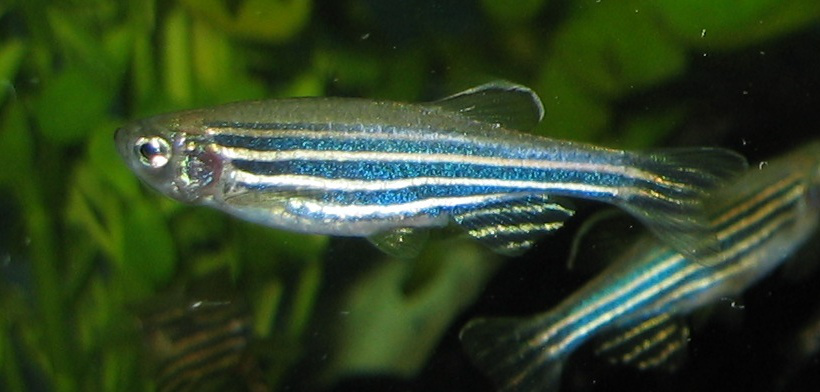
\includegraphics[width=0.99\textwidth]{pictures/zebrafishPic}
\end{center}
\caption{Mature zebra fish: approximatively 2.5cm long (source: \href{http://en.wikipedia.org/wiki/File:Zebrafisch.jpg}{Wikipedia})}
\label{fig:ZebraPic}
\end{figure}

\section{Systems Biology}

With the completion of the genome projects~\cite{}, the stage is now set for a
more complete understanding of how animals are created. Biologists now have
access to the complete sequence of DNA that encodes the blueprint of life for
many animals including human, mouse, zebrafish, and fruit
fly~\cite{[2][3][4][5]} \TODO{refe?}The challenge is now understanding how this
code functions. The problem however is that the only thing that biologists can
currently reliably predict from the genomic code is which parts can be
transcribed and translated into protein. Biologists cannot accurately predict
when and where a protein will be expressed, how a protein will
function once it is created, and the interaction between expressed proteins that
allow them to form functional genetic circuits. Thus, although the genome
projects have given us the complete code for constructing many organisms, the
only part of the code biologists can currently read is the parts list. The
challenge is understanding how all these parts fit together to form molecular
circuits, how these circuits process information to regulate the behavior of
cells, and how the behavior of cells is orchestrated to generate functional form
as in \emph{embryogenesis}. This post-genomic endeavor has come to be called
\emph{systems biology}.\\

Although systems biology grew out of the “-omics” field which made heavy use of 
in vitro biochemical approaches (e.g. sequencing, microarrays, and proteomics),
\textit{in-vivo} imaging is becoming an increasingly powerful tool for
systems biology. \textit{In-vivo} imaging is advantageous over
biochemical approaches for doing systems biology:

\begin{itemize}
 \item Biological circuits function at the single cell level. Microscopic
imaging easily achieves this resolution while in-vitro techniques do not.
 \item Biological circuits function over time. With imaging, different
components of a biological circuit can be labeled using different colors of
fluorescent proteins and the dynamics of the circuit monitored non-invasively
with time-lapse fluorescent imaging as the circuit functions in an intact
system. In vitro biochemical approaches typically require the tissue to
be destroyed in order to be assayed which precludes longitudinal analysis.
 \item the quantitative amounts of components in a biological circuit are
important for its function. Fluorescent imaging can accurately quantitate the
levels of molecular components even at the protein level through the use of
fluorescent protein (e.g. GFP) fusions. Omic approaches are typically less
quantitative and focus at the DNA or RNA level which is less relevant.
 \item the anatomical context of biological circuits is essential for
determining their function; the use of spatial cues to generate different cell
types in different places is a fundamental aspect of development. In vivo
imaging can capture data from intact animals preserving its anatomical context.
In vitro approaches typically grind up the tissue to assay it, thus destroying
its anatomy.
\end{itemize}

%%%%%%%%%%%%%%%%%%%%%%%%%%%%%%%%%%%%%%%%%%%%%%%%%%%%%%%%%%%%%%%%%%%%%%%%%%%%%%%
%%%%%%%%%%%%%%%%%%%%%%%%%%%%%%%%%%%%%%%%%%%%%%%%%%%%%%%%%%%%%%%%%%%%%%%%%%%%%%%
%%%%%%%%%%%%%%%%%%%%%%%%%%%%%%%%%%%%%%%%%%%%%%%%%%%%%%%%%%%%%%%%%%%%%%%%%%%%%%%

\section{Zebrafish: one sytem of high interest for Systems-Biology}

Zebrafish (Danio rerio) is a small, freshwater, tropical fish commonly available
in pet stores (see figure~\ref{}). It has become a popular model system for the
study of genetics and development in the last 2 decades and there are now
many labs worldwide that study it. There have been several
large-scale mutagenesis screens caried out in zebrafish and its genome has been
largely sequenced. Zebrafish has the advantages of fruit fly in that it
is amenable to forward genetic screens, but unlike fruit fly, zebrafish is a
vertebrate so is much more relevant to humans. Another huge advantage
of zebrafish is its suitability for imaging. Zebrafish embryos are transparent,
small, develop freely outside their mother, and develop directly from egg to
adult without any larval stages. This means that a zebrafish egg can be placed
under a microscope and continuously imaged throughout embryogenesis. This would
be impossible with a mouse which develop inside its mother, with a frog
(Xenopus) egg which is opaque, or with a fruit fly (Drosophila) which has
several larval/pupal stages and is opaque.

%%%%%%%%%%%%%%%%%%%%%%%%%%%%%%%%%%%%%%%%%%%%%%%%%%%%%%%%%%%%%%%%%%%%%%%%%%%%%%%
%%%%%%%%%%%%%%%%%%%%%%%%%%%%%%%%%%%%%%%%%%%%%%%%%%%%%%%%%%%%%%%%%%%%%%%%%%%%%%%
%%%%%%%%%%%%%%%%%%%%%%%%%%%%%%%%%%%%%%%%%%%%%%%%%%%%%%%%%%%%%%%%%%%%%%%%%%%%%%%

\section{In-toto imaging: one technique of interest for Systems-Biology}

The goal of in toto imaging is to image and track every single cell in a
developing tissue, organ, or eventually
whole embryo~\cite{megason2003digitizing}. This technique will provide
significant outcomes in a complete understanding of the cellular basis of
development through the construction of complete lineage trees\footnote{First
results on early zebrafish embryo~\cite{SCIENCE-PAPER} show the immense impact
on the scientific community of such a technique.}. There are several steps to in
toto imaging.\\

The embryos must first be labeled with “segmentation markers” which allow all
the cells to be segmented. Additionally embryos can be labeled with additional
markers to reveal RNA or protein expression. The next step is to acquire 3D+t
image sets using confocal or 2-photon fluorescent microscopy. And the final step
is processing the often very large image sets to segment out all the cell
trajectories and to extract quantitative, cell-centric data.

\subsection{Embryo Labeling}

The living embryos must be labeled with fluorescent markers and imaged with
time-lapse technique. Biologists must use vital labels such as Green
Fluorescent Protein (GFP), or other available Fluorescence Proteins (FPs) across
the visible spectrum. Since FPs are proteins rather than organically synthesized
small molecule dyes, FPs can be endogenously expressed by transgenic organisms
and are open to all the power of genetic engineering.\\

There are 2 basic uses of markers for in toto imaging: segmentation and
expression.
\begin{itemize}
 \item Segmentation markers allow the cells to be segmented in space,
across time, and across cell-division. Biologists, at the Megason Lab, typically
use a histone-FP of one color (e.g. histone-cerulean) and a membrane-localized
FP of another color (e.g. membrane-mCherry). This combination would generate
embryos in which every nuclei is green and all the cell membranes are red~(see
figure~\ref{}).
 \item Expression markers refer to whatever else is being marked such that it
can be digitized with in toto imaging. For example, transgenic fish can be made
that express a fluorescent protein wherever some gene is normally expressed
during development.
\end{itemize}

%%%%%%%%%%%%%%%%%%%%%%%%%%%%%%%%%%%%%%%%%%%%%%%%%%%%%%%%%%%%%%%%%%%%%%%%%%%%%%%
%%%%%%%%%%%%%%%%%%%%%%%%%%%%%%%%%%%%%%%%%%%%%%%%%%%%%%%%%%%%%%%%%%%%%%%%%%%%%%%
%%%%%%%%%%%%%%%%%%%%%%%%%%%%%%%%%%%%%%%%%%%%%%%%%%%%%%%%%%%%%%%%%%%%%%%%%%%%%%%

\subsection{Image acquisition}

\subsubsection{Requirements}

In toto imaging tracks cells during development only by the correspondence of
cells from frame to frame. This is quite different than traditional fate mapping
in developmental biology where only a small subset of cells is labeled at one
stage of development and the location of their progeny is observed at a
later stage. In toto imaging thus requires images that have high enough
resolution in space to resolve all the cells (this requires $\approx
1 \mu$m resolution) and high enough resolution in time to not lose track of
moving and dividing cells (this requires $\approx 2$ min time resolution). In
addition to high resolution, in toto imaging also requires complete coverage.
All the cells of interest must be continuously imaged in order to be tracked; if
cells leave the field of view then their lineage cannot be completely tracked.

\subsubsection{Equipment}

Achieving both high spatial and temporal resolution as well as complete coverage
can be achieved through the use of time-lapse confocal or 2-photon microscopy.
Confocal microscopy~(see figure~\ref{fig:ConfocalPrinciple}) uses a pinhole to
eliminate out of focus light whereas 2-photon microscopy only excites
fluorescence in the focal plane.

Thus both techniques allow thin (1$\mu$m) optical sections of fluorescent
samples to be captured. By imaging at a series of focal planes, stacks of
optical sections can be captured to generate a volumetric image and this can be
repeated over time to generate 3D+t images. The axial (z) resolution with these
techniques is typically around 5-fold less than the planar (xy) resolution so
the volumetric images are anisotropic. Confocal imaging provides 2-fold higer
resolution than 2-photon imaging but has a depth penetration limit of  150 um.
2-photon imaging can image all the way through a zebrafish embryo and has
reduced phototoxicity to the embryo and photobleaching of the fluorescent
labels.\\

Both acquisition techniques have been assembled in the Megasaon Lab from a
Zeiss 710 NLO (figure~\ref{fig:MicMegason}).


\begin{figure}[htb]
\begin{center}
\leavevmode
 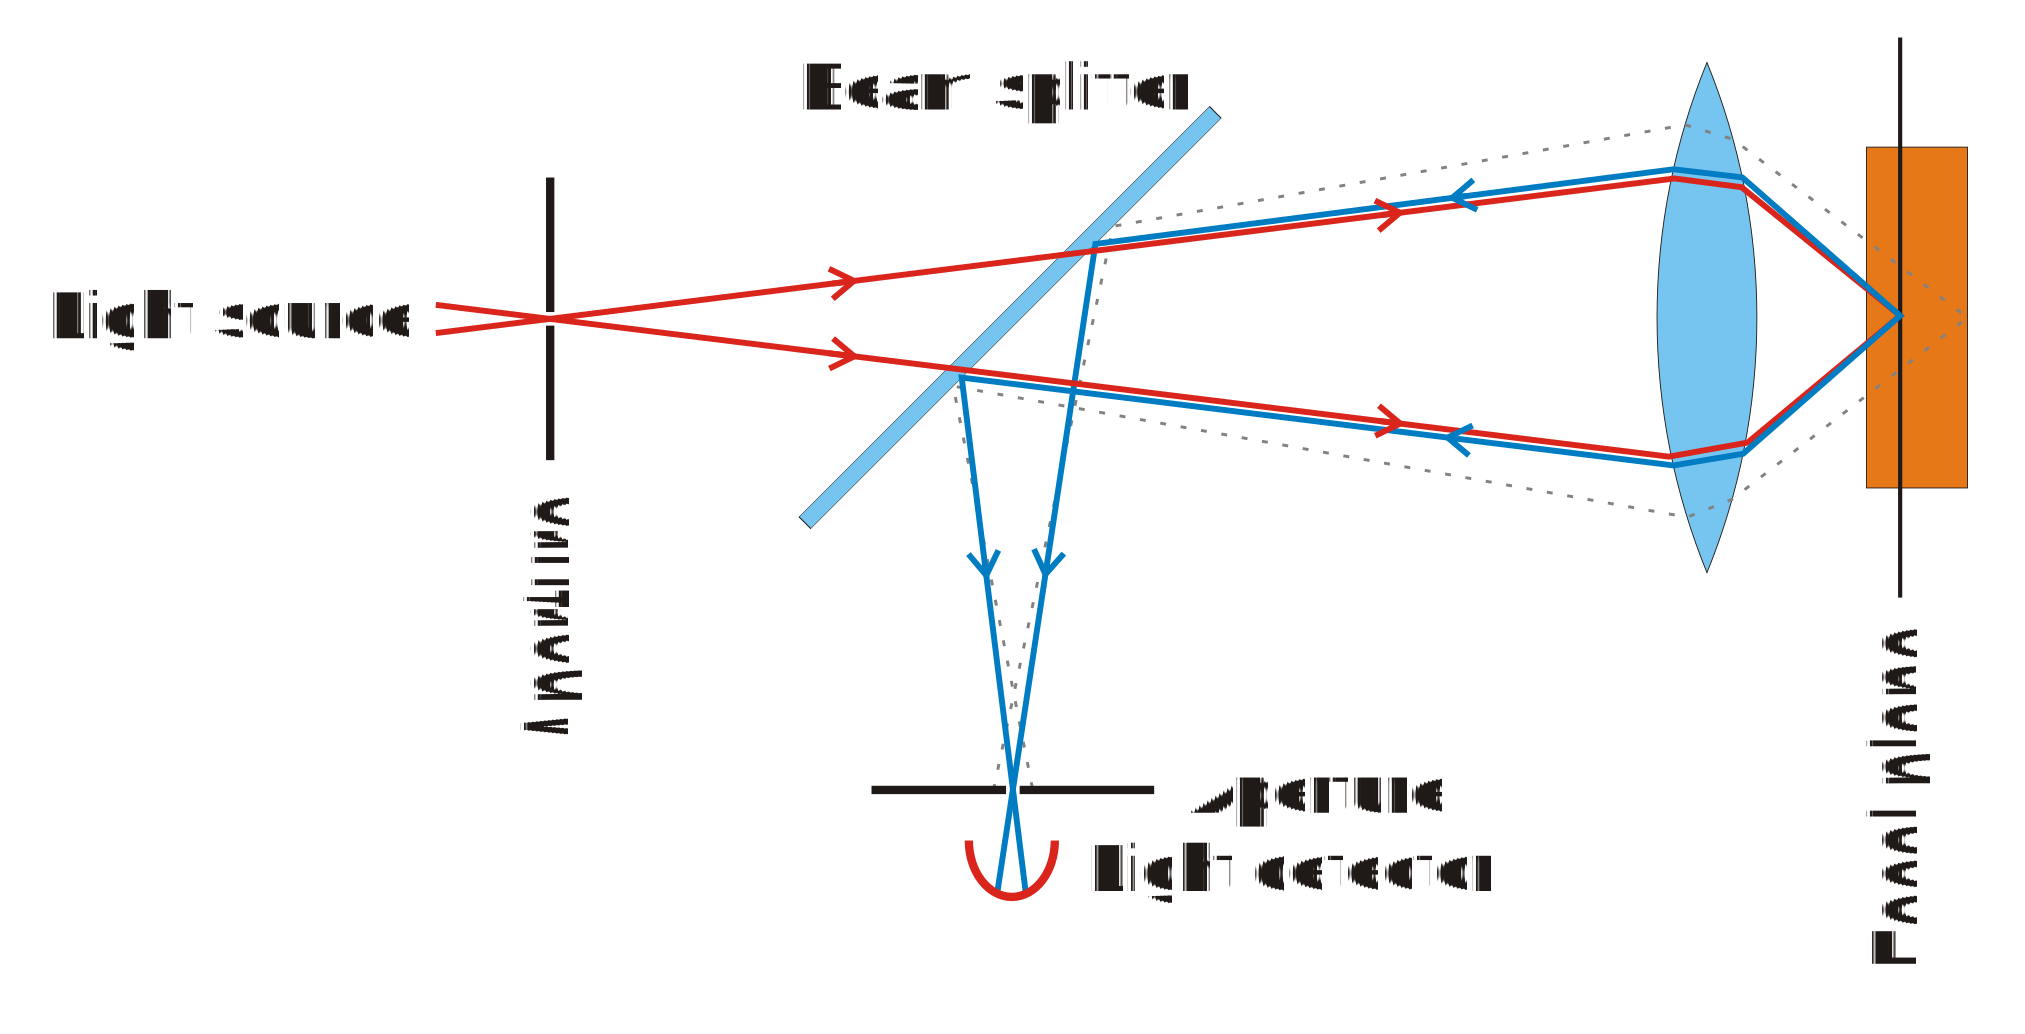
\includegraphics[width=0.95\textwidth]{pictures/ConfocalPrinciple}
\end{center}
\caption{Confocal microscope principle
(source:\href{http://en.wikipedia.org/wiki/File:Confocalprinciple.svg}{Wikipedia
})}
\label{fig:ConfocalPrinciple}
\end{figure}

\begin{figure}[htb]
\begin{center}
\leavevmode
 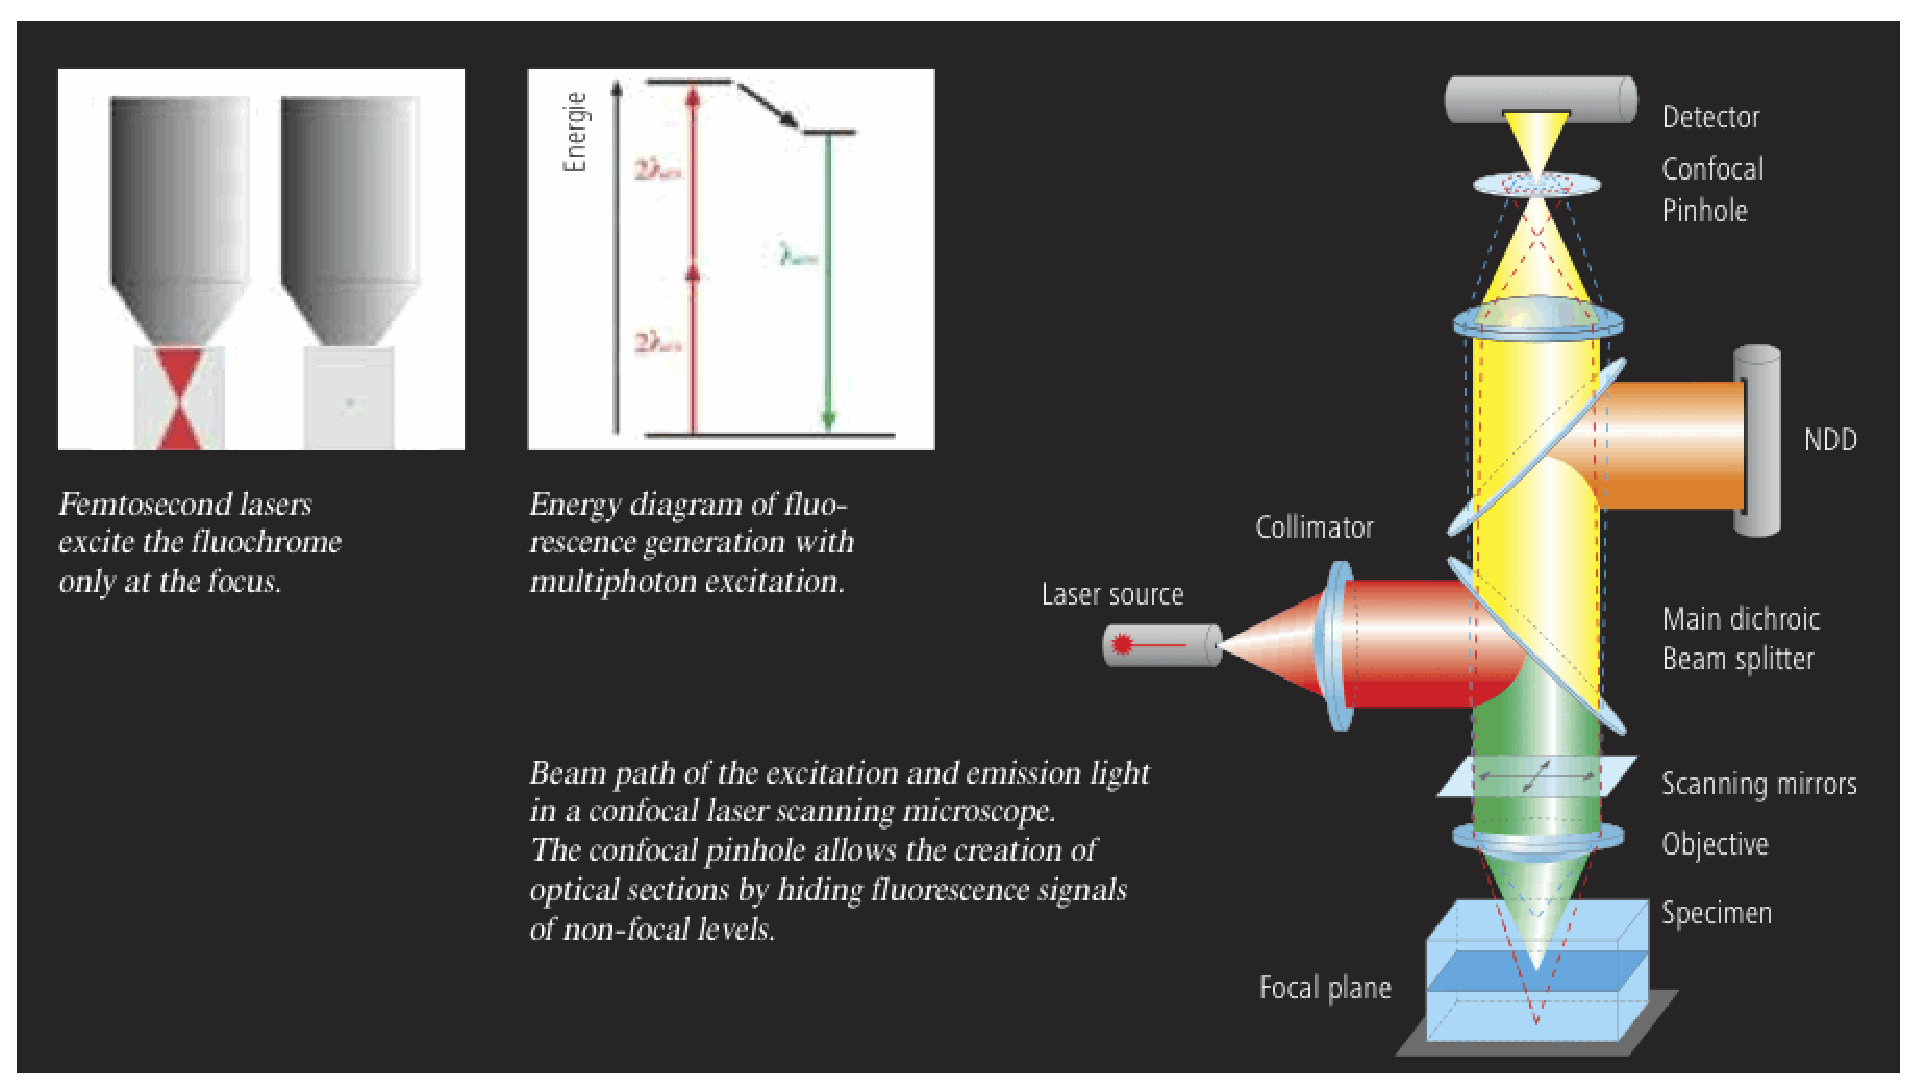
\includegraphics[width=0.95\textwidth]{pictures/ConfocalZeissPrinciple}
\end{center}
\caption{2-photon confocal microscope principle (Zeiss documentation)}
\label{fig:Confocal2photonsPrinciple}
\end{figure}

\begin{figure}[htb]
\begin{center}
\leavevmode
 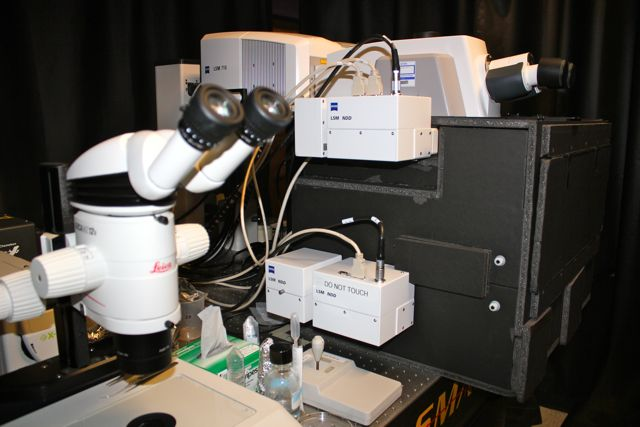
\includegraphics[width=0.95\textwidth]{pictures/PICmicroscope}
\end{center}
\caption{2-photon confocal microscope Zeiss 710 NLO in service in the Megason
Lab}
\label{fig:MicMegason}
\end{figure}

%%%%%%%%%%%%%%%%%%%%%%%%%%%%%%%%%%%%%%%%%%%%%%%%%%%%%%%%%%%%%%%%%%%%%%%%%%%%%%%
%%%%%%%%%%%%%%%%%%%%%%%%%%%%%%%%%%%%%%%%%%%%%%%%%%%%%%%%%%%%%%%%%%%%%%%%%%%%%%%
%%%%%%%%%%%%%%%%%%%%%%%%%%%%%%%%%%%%%%%%%%%%%%%%%%%%%%%%%%%%%%%%%%%%%%%%%%%%%%%

\subsection{Image Processing}

After the embryos have been labelled and imaged, the final challenge of in toto
imaging is image processing. The goal of image processing is to track all the
cell movements and divisions to generate cell lineage trees, to define the
boundaries of all cells and their compartments (nucleus, cytoplasm, membrane,
extracellular space), and to quantize the level of fluorescence within each
cell and subcellular compartment.\\

In order to process all the acquired data, an image processing team of
is working on the next platform of microscopy images analysis: {\gofigure}.
Their goal is to create a very accessible "cross-platform"\footnote{In
computing, cross-platform, or multi-platform, is
an attribute conferred to computer software or computing methods and concepts
that are implemented and inter-operate on multiple operating systems and
hardware.}, "open-source"\footnote{of or
relating to or being computer software for which
the source code is freely available, but which use may be restricted by a
license.}, freely distributed, application with a high quality code, for
biologists to process their data and for computer scientists and image
processing specialists the opportunity to promote their methods.

%%%%%%%%%%%%%%%%%%%%%%%%%%%%%%%%%%%%%%%%%%%%%%%%%%%%%%%%%%%%%%%%%%%%%%%%%%%%%%%
%%%%%%%%%%%%%%%%%%%%%%%%%%%%%%%%%%%%%%%%%%%%%%%%%%%%%%%%%%%%%%%%%%%%%%%%%%%%%%%
%%%%%%%%%%%%%%%%%%%%%%%%%%%%%%%%%%%%%%%%%%%%%%%%%%%%%%%%%%%%%%%%%%%%%%%%%%%%%%%



%
%\begin{figure}[htb]
%\begin{center}
%\leavevmode
%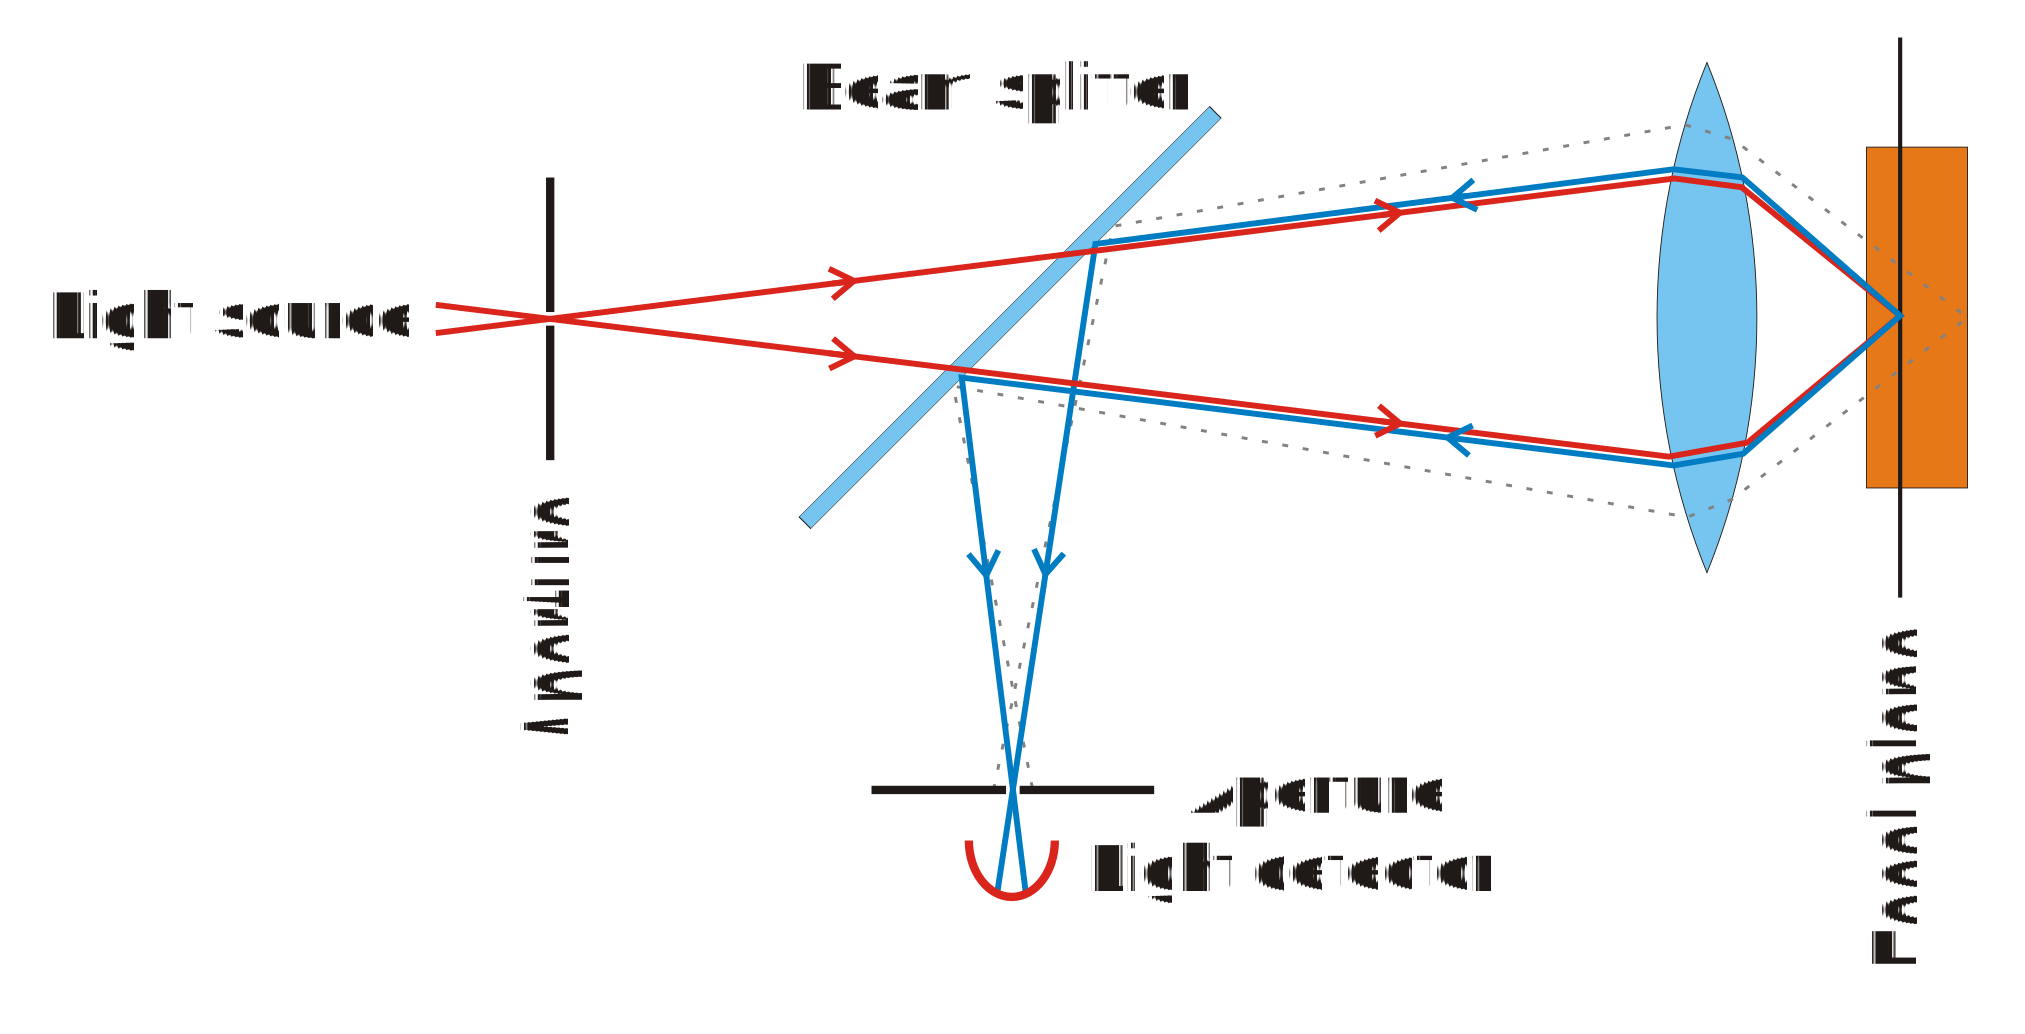
\includegraphics[width=0.95\textwidth]{pictures/ConfocalPrinciple}
%\end{center}
%\caption{Confocal microscope principle (source:\href{http://en.wikipedia.org/wiki/File:Confocalprinciple.svg}{Wikipedia})}
%\label{fig:ConfocalPrinciple}
%\end{figure}
%
%\begin{figure}[htb]
%\begin{center}
%\leavevmode
% 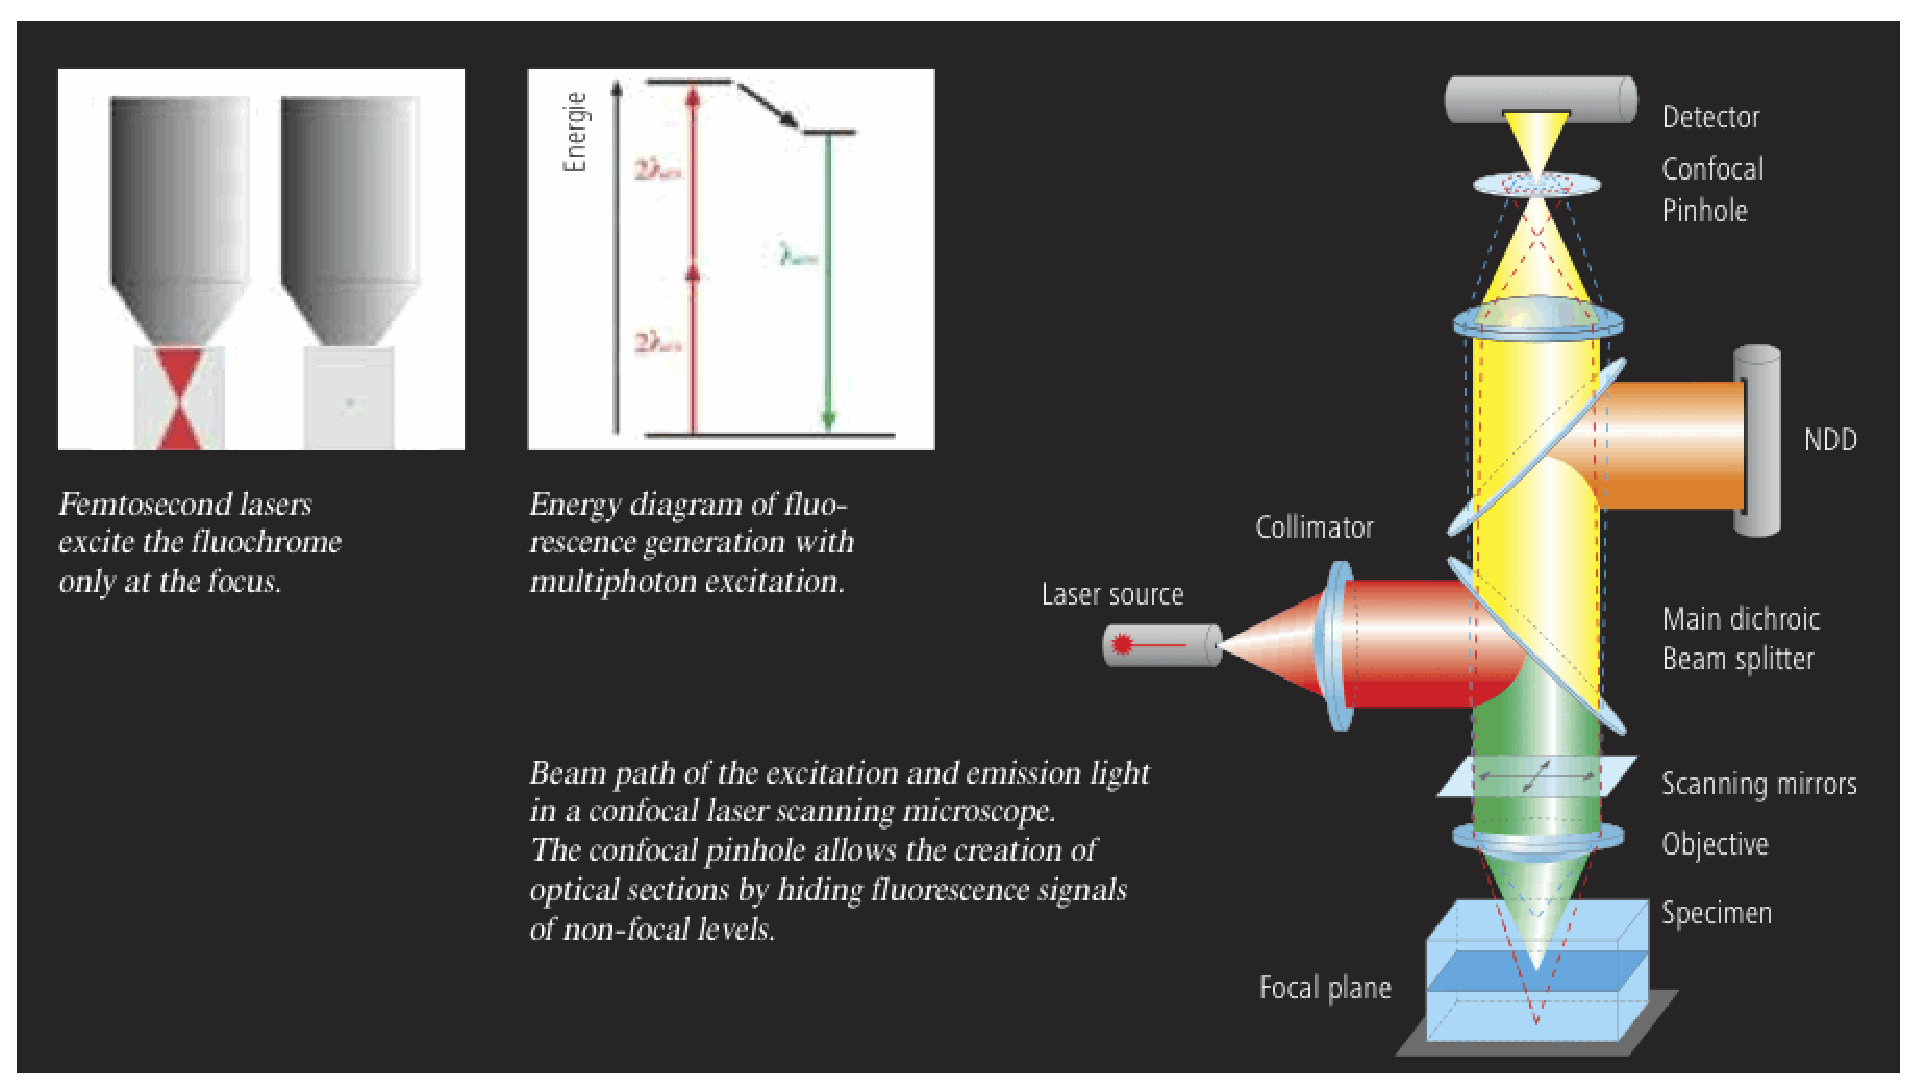
\includegraphics[width=0.95\textwidth]{pictures/ConfocalZeissPrinciple}
%\end{center}
%\caption{2-photon confocal microscope principle (Zeiss documentation)}
%\label{fig:Confocal2photonsPrinciple}
%\end{figure}
%
%\begin{figure}[htb]
%\begin{center}
%\leavevmode
%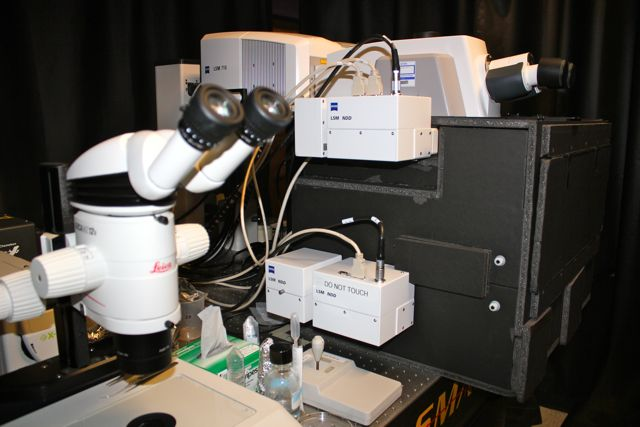
\includegraphics[width=0.95\textwidth]{pictures/PICmicroscope}
%\end{center}
%\caption{2-photon confocal microscope Zeiss 710 NLO in service in the Megason Lab}
%\label{fig:MicMegason}
%\end{figure}


\section{Problematic}


As discussed previously, membrane segmentation is an important step in the process of understanding the development of an embryo.
Indeed, membrane provide useful informations on the local connectivity between cells, and on local characteristics of a given cell (like volume, shape information...).
Segmenting cell membrane is a challenging problem (see section~\ref{}): data are incomplete, quite noisy, 3D and anisotropic.

Due to the physics of the image acquisition, data are never complete and thus any segmentation technique need serious prior to properly extract cell membrane.
An assumption based on biological knowledge is that each nucleus belongs to one cell, and is inside the space enclosed by the cell membrane.
Two important points should be pointed out from this assumption:
\begin{itemize}
    \item cell membranes are closed
    \item cell nuclei center are inside
\end{itemize}

Under this assumption, correctly detecting nuclei is thus really important to extract cell membrane in images.
In my thesis, I will focus on cell nuclei detection in order to efficiently extract and segment cell membranes.
In the rest of the document, I shall first present the data to be processed, and existing method for nuclei segmentation;
then, I will introduce my technique in which I make use of information from the nuclei channel and the membrane channel;
I will present results of my method on synthetic data sets, as well as on real data sets, with validation and comparison with existing methods.
Finally, I will conclude and suggest some improvements to my method and some future plans in order to use this method for segmenting cell membranes. 


\input{chapters/Stateoftheart}


\chapter{My Proposal}
\label{chapt:proposal}


As section~\ref{setc:ChallengesData} demonstrates, the Megason lab's datasets are hard to proceed. That forces us to find innovative solution for problems that may seem simple at first glance.

This chapter describes the new method we proposed in order to solve the nuclei detection problem. This new method uses a different approaches based on the membrane information as principal and not complimentary information. We shall first introduce the theorical concepts of this method, and prove its functioning on a simple dataset.


All the papers we have been reading take advantage of the nuclei channel information, but none of them takes advantage of the membrane channel.
This channel provides capital information, especially in the case of stuck nuclei, where most common detection method fail.
Indeed, the membrane can separate the different nuclei.
We propose here a method using the membrane information in an original way.



%%%%%%%%%%%%%%%%%%%%%%%%%%%%%%%%%%%%%%%%%%%%%%%%%%%%%%%%%%%%%%%%%%%%%%%%%%%%%%%
%%%%%%%%%%%%%%%%%%%%%%%%%%%%%%%%%%%%%%%%%%%%%%%%%%%%%%%%%%%%%%%%%%%%%%%%%%%%%%%
%%%%%%%%%%%%%%%%%%%%%%%%%%%%%%%%%%%%%%%%%%%%%%%%%%%%%%%%%%%%%%%%%%%%%%%%%%%%%%%


\section{Preliminaries}
\label{sect:definitions}
We present here the mathematical concepts used by the proposal.


\subsection{Euclidean distance map}
\label{subsec:EuclDistMapDef}
Let \( I : \Omega \subset \mathbb{Z}^3 \leftarrow \{0,1\} \) be a binary image where the domain \({\Omega}\) is convex, in particular, \( \Omega  = \{1,{\dots},n\}{\times}\{1,{\dots},n\}{\times}\{1,{\dots},n\} \). By convention, 0 is associated to black and 1 to white, Hence we have an object \({\mathcal{O}}\) represented by all the white pixels:\\
\begin{center}
\( {\mathcal{O}} = p \in \Omega \mid I(p)=1 \)
\end{center}

The set \({\mathcal{O}}\) is called object or foreground and can consist of any subset of the image domain, including disjoint sets.
The elements of its complement,\(\overline{\mathcal{O}}\), the set of black pixels in \({\Omega}\), are called background.
\begin{itemize}
\item For two pixels, \({p : (p_x, p_y, p_z)}\) , and \({q : (q_x, q_y, q_z)}\), the Euclidean distance is given by : 
\[
d(p,q) = \sqrt{ (p_x-q_x)^{2}+(p_y-q_y)^{2}+(p_z-q_z)^{2} }
\]
%
\item The distance transform (DT) is the transformation that generates a map \({D}\) whose value in each pixel \({p}\) is the smallest distance from this pixel to \(\overline{\mathcal{O}}\):
\[
D(p) := min\{ d(p,q) \mid q \in \overline{\mathcal{O}}\} = min\{ d(p,q) \mid I(q) = 0 \}
\]
The image \({D}\) is called the distance map of \({I}\).
\end{itemize}


\subsection{Voronoi diagram}

We define here the \emph{point-wise Voronoi diagram} (VD) and related concepts.
The \emph{Voronoi region} (VR) of an interest point is the set of points strictly closer to it than to any other interest point. The \emph{Voronoi element} closest to a given pixel \({p}\) is denoted by {\( VS(p) \)}. In case \({p}\) has two or more closest \emph{sites}, one of them is arbitrarily chosen to be {\( VS(p) \)}. By definition, the point-wise Voronoi diagram is the set of points closest to one or more \emph{sites}, that is, the points not in any Voronoi region. A Voronoi partition is the collection of the VRs of all \emph{sites} or \emph{seeds}. To build the partition, each point of the VD is arbitrarily attributed to the VR of one of the \emph{sites} minimally equidistant to it.
The Voronoi partition can be represented by the label map, where each VS has an associated label (a number) that identifies this VS and pixels of its VR. The label map is formally defined as:

\[
Label : \Omega \rightarrow \{ 1,{\dots},n_s \}  \\
p \rightarrow Label(p) = \{ Label(q) \mid q = VS(p) \}
\]
where \({n_s}\) is the number of \emph{sites} (and of VRs).

%\xmapsto


\subsection{Centroid}

The \emph{centroid} \({c_\mathcal{O}}\) of an object \({\mathcal{O}}\) is defined as:
\[
c_O :=  \sum_{p \in {O}} \frac{p}{Card(O)}
\]


\subsection{Assumptions}

\begin{figure}[h]
\begin{center}
\leavevmode
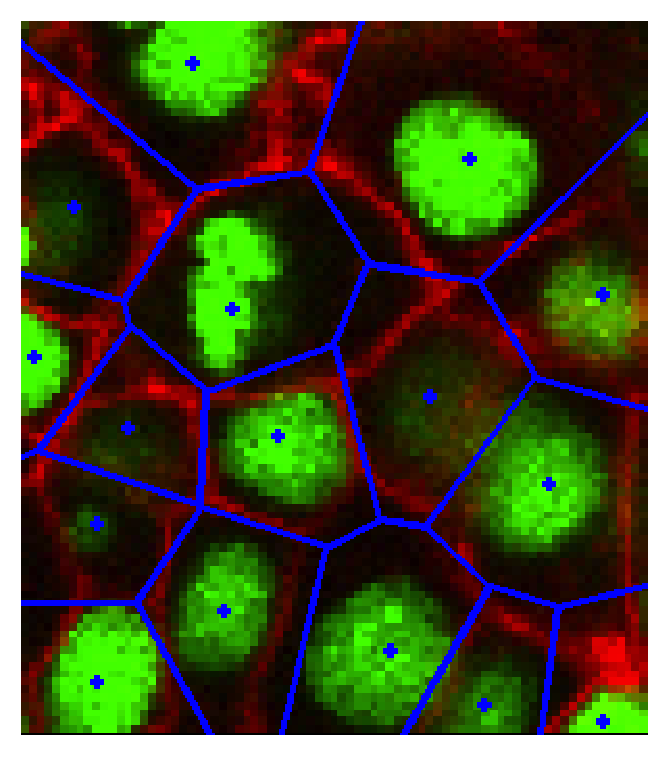
\includegraphics[width=0.5\textwidth]{pictures/voronoiExample2D}
\end{center}
\caption{Boundary of Voronoi regions (blue) generated from each cell nuclei (green), with the membrane (red). The Voronoi  diagram was generated in 2D.}
\label{fig:voronoiExample2D}
\end{figure}

\begin{figure}[h]
\begin{center}
\leavevmode
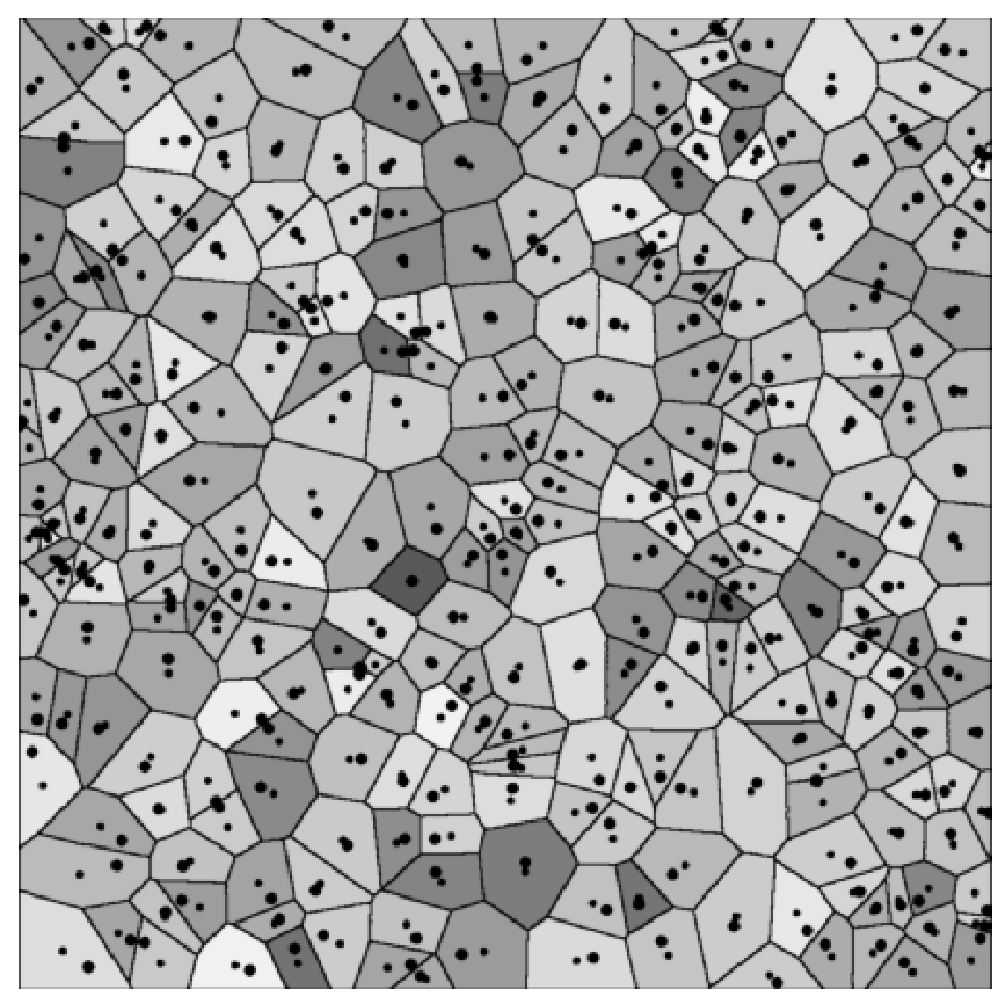
\includegraphics[width=0.5\textwidth]{pictures/centroidVoronoi}
\end{center}
\caption{Voronoi diagram with \emph{sites} (large dots) and centroids (small dots). Image from~\cite{Secord02randommarks}.}
\label{fig:centroidVoronoi}
\end{figure}


Several article make use of \emph{Voronoi diagrams} to model the membrane of cells~\cite{luengo2008can,yu2010evolving}.
But the membrane is also around each nuclei. So the membrane channel provides us with information about nuclei positions.
We based our algorithm on two assumptions :
\begin{itemize}
\item The membrane can be considered as a \emph{Voronoi diagram}.
\item Nuclei are in the center of cells, and correspond to the \emph{sites} of the \emph{Voronoi diagram}.
\end{itemize}
We can see figure~\ref{fig:voronoiExample2D}, that the membrane can be approximated by a \emph{Voronoi diagram} centred in each nucleus.
From this, we can use the membrane channel and consider it as a \emph{Voronoi tessellation}.


%%%%%%%%%%%%%%%%%%%%%%%%%%%%%%%%%%%%%%%%%%%%%%%%%%%%%%%%%%%%%%%%%%%%%%%%%%%%%%%
%%%%%%%%%%%%%%%%%%%%%%%%%%%%%%%%%%%%%%%%%%%%%%%%%%%%%%%%%%%%%%%%%%%%%%%%%%%%%%%
%%%%%%%%%%%%%%%%%%%%%%%%%%%%%%%%%%%%%%%%%%%%%%%%%%%%%%%%%%%%%%%%%%%%%%%%%%%%%%%


\section{Method}

\begin{figure}[h]
\begin{center}
\leavevmode
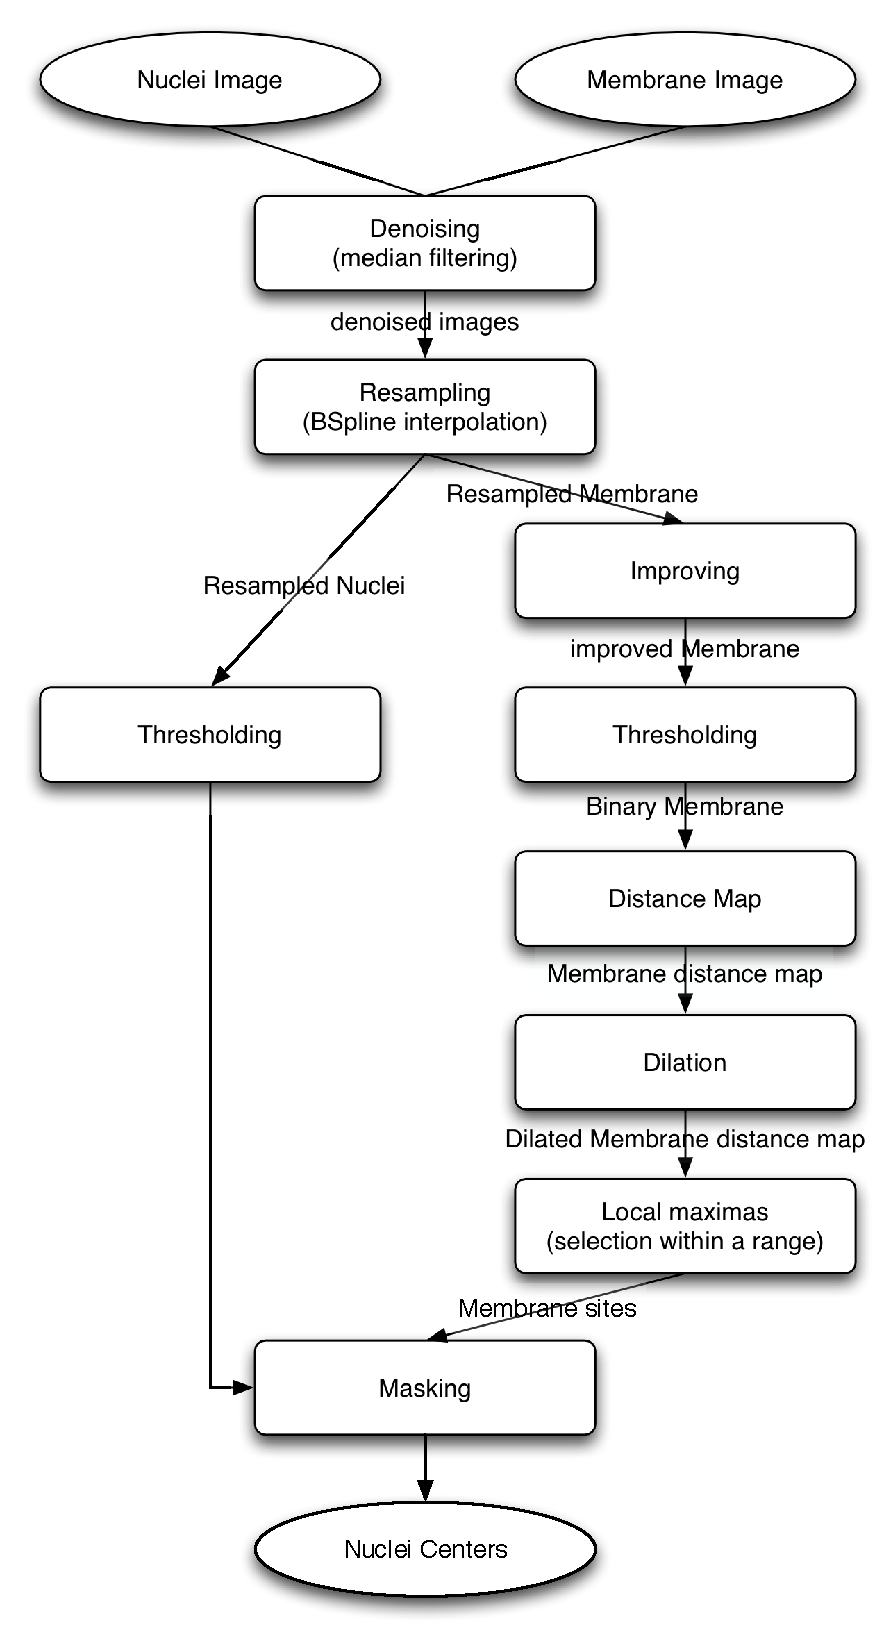
\includegraphics[height=0.87\textheight]{pictures/proposalFlowchart}
\end{center}
\caption{Flowchart of the proposed algorithm.}
\label{fig:propFlowchart}
\end{figure}

As defined in \ref{sect:definitions},the \emph{Voronoi cells} (or VRs) are constituted by all the points closer to the \emph{site} of the cell than any other \emph{site}.

We have a damaged information about the boundaries of the VRs. In order to reconstruct a \emph{Voronoi diagram},
 we consider that the cell membrane represents a \emph{centroidal Voronoi tessellation} (see figure~\ref{fig:centroidVoronoi}): we locate the centroid of each VR, and from that, estimate the position of the nuclei.
 
We use the distance map information to find a subset of the VR within the damaged membrane cells.
Using this distance information, we find an approximation of the VR (approximate VR), and we use the centroid of this region to approximate the location of the \emph{site}.
We will first describe our algorithm. We will then introduce the difficulties we encountered (see section~\ref{sect:difficultiesTheory}), and prove that even with noisy and incomplete membrane information, we are able to find the approximate position of the \emph{sites}.


\subsection{Algorithm pipeline}

It is clear that for most image processing problems, a series of transformation is needed in order to be able to work with the data.
Inspired by the described articles, I designed an image processing pipeline adapted to our data.
I describe here the image processing pipeline for the new algorithm, and the improvements of the existing nuclei segmentation pipeline
\begin{description}
  \item[Denoising: ] We first process the membrane and the nuclei channel with a median filter. The median filter's structuring element is a disk of radius one third of the radius of a nuclei, for the nuclei channel, and one third of the thickness of the membrane for the membrane channel.
  We process the images before resampling, as the resampling on the z stack spreads noisy points, invalidating the median filter's use.
%
%
  \item[Images Resampling: ] As in~\cite{li20073}, our images are anisotropic : they are very high resolution in xy, and very low resolution in z, as shown by the
  table~\ref{tab:DataSizes}, and the figure~\ref{fig:anisotropy}.
  We don't need this much information in xy, as algorithms are computationally expensive, and we want to keep a reasonable processing time.
  But, we need a higher resolution in z.
  For that purpose, we resample our images, using a BSpline interpolation of order 5.
  This technique provides us with an isotropic dataset of spacing 0.4um, that can easily be
  processed by the other filters. The interpolation, in the z direction, partially reconstructs the membrane.
%
%
  \item[Nuclei binary mask: ] We threshold the nuclei image to keep a rough binary mask in which the nuclei are present (see figure~\ref{fig:propNucleiMask}).
  The thresholds are chosen empirically after an analysis of the histogram of the nuclei images.
%  
%
%  
  \item[Distance map creation: ] We then process the resampled and denoised membrane channel with Kishore's membrane reconstruction filter.
  The resultant membrane is thresholded to get a binary image from which we compute a distance map (see figure~\ref{fig:propDistance})
  using the algorithm proposed by Maurer Jr {\etal}~\cite{maurer2003linear}, as it is the fastest for big binary images with complex structures according to~\cite{distanceMapReview}.
  The threshold values are empirically determined.
%  
%
%
  \item[Approximate Voronoi Cell extraction: ] Then, we threshold the distance map with a threshold value of one third of a nuclei radius.
  From this thresholding, we get a set of regions located inside each cell : the approximate VRs (see figure~\ref{fig:propThresholdedDistanceMap}).
  If the assumption that holes are much smaller than nuclei radius is correct, those regions should not touch because the distance map should not have high value between different VRs. We use a labelling procedure, to separate each of these regions.
%
%
  \item[Nuclei detection: ] We finally locate the centroid of each approximate VR and output this result as cell nuclei detection.
%  
%
%
\end{description}


\begin{figure}[h]
  \centering
\subfloat[][]{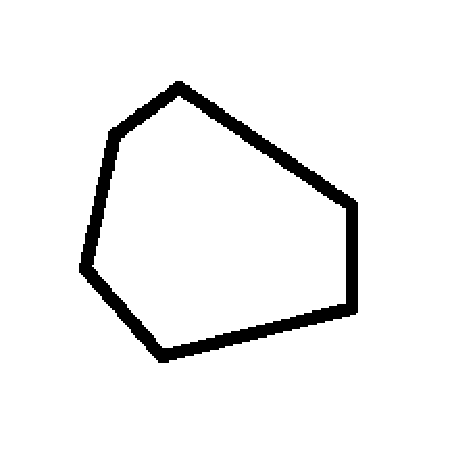
\includegraphics[width=0.33\textwidth, height=0.33\textwidth]{pictures/theoryComplete}\label{fig:theoryComplete}}
\subfloat[][]{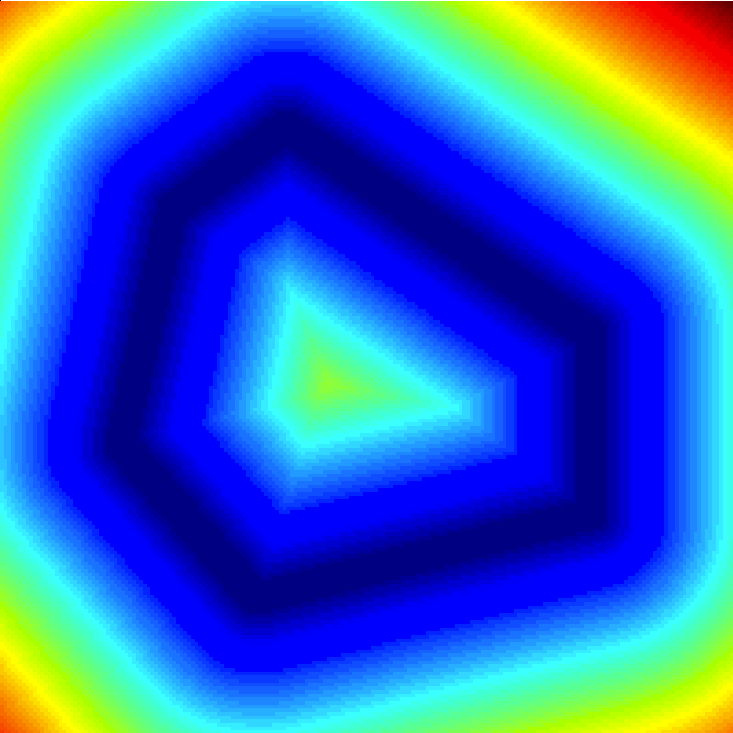
\includegraphics[width=0.33\textwidth, height=0.33\textwidth]{pictures/theoryCompleteDistance}\label{fig:theoryCompleteDistance}}
\subfloat[][]{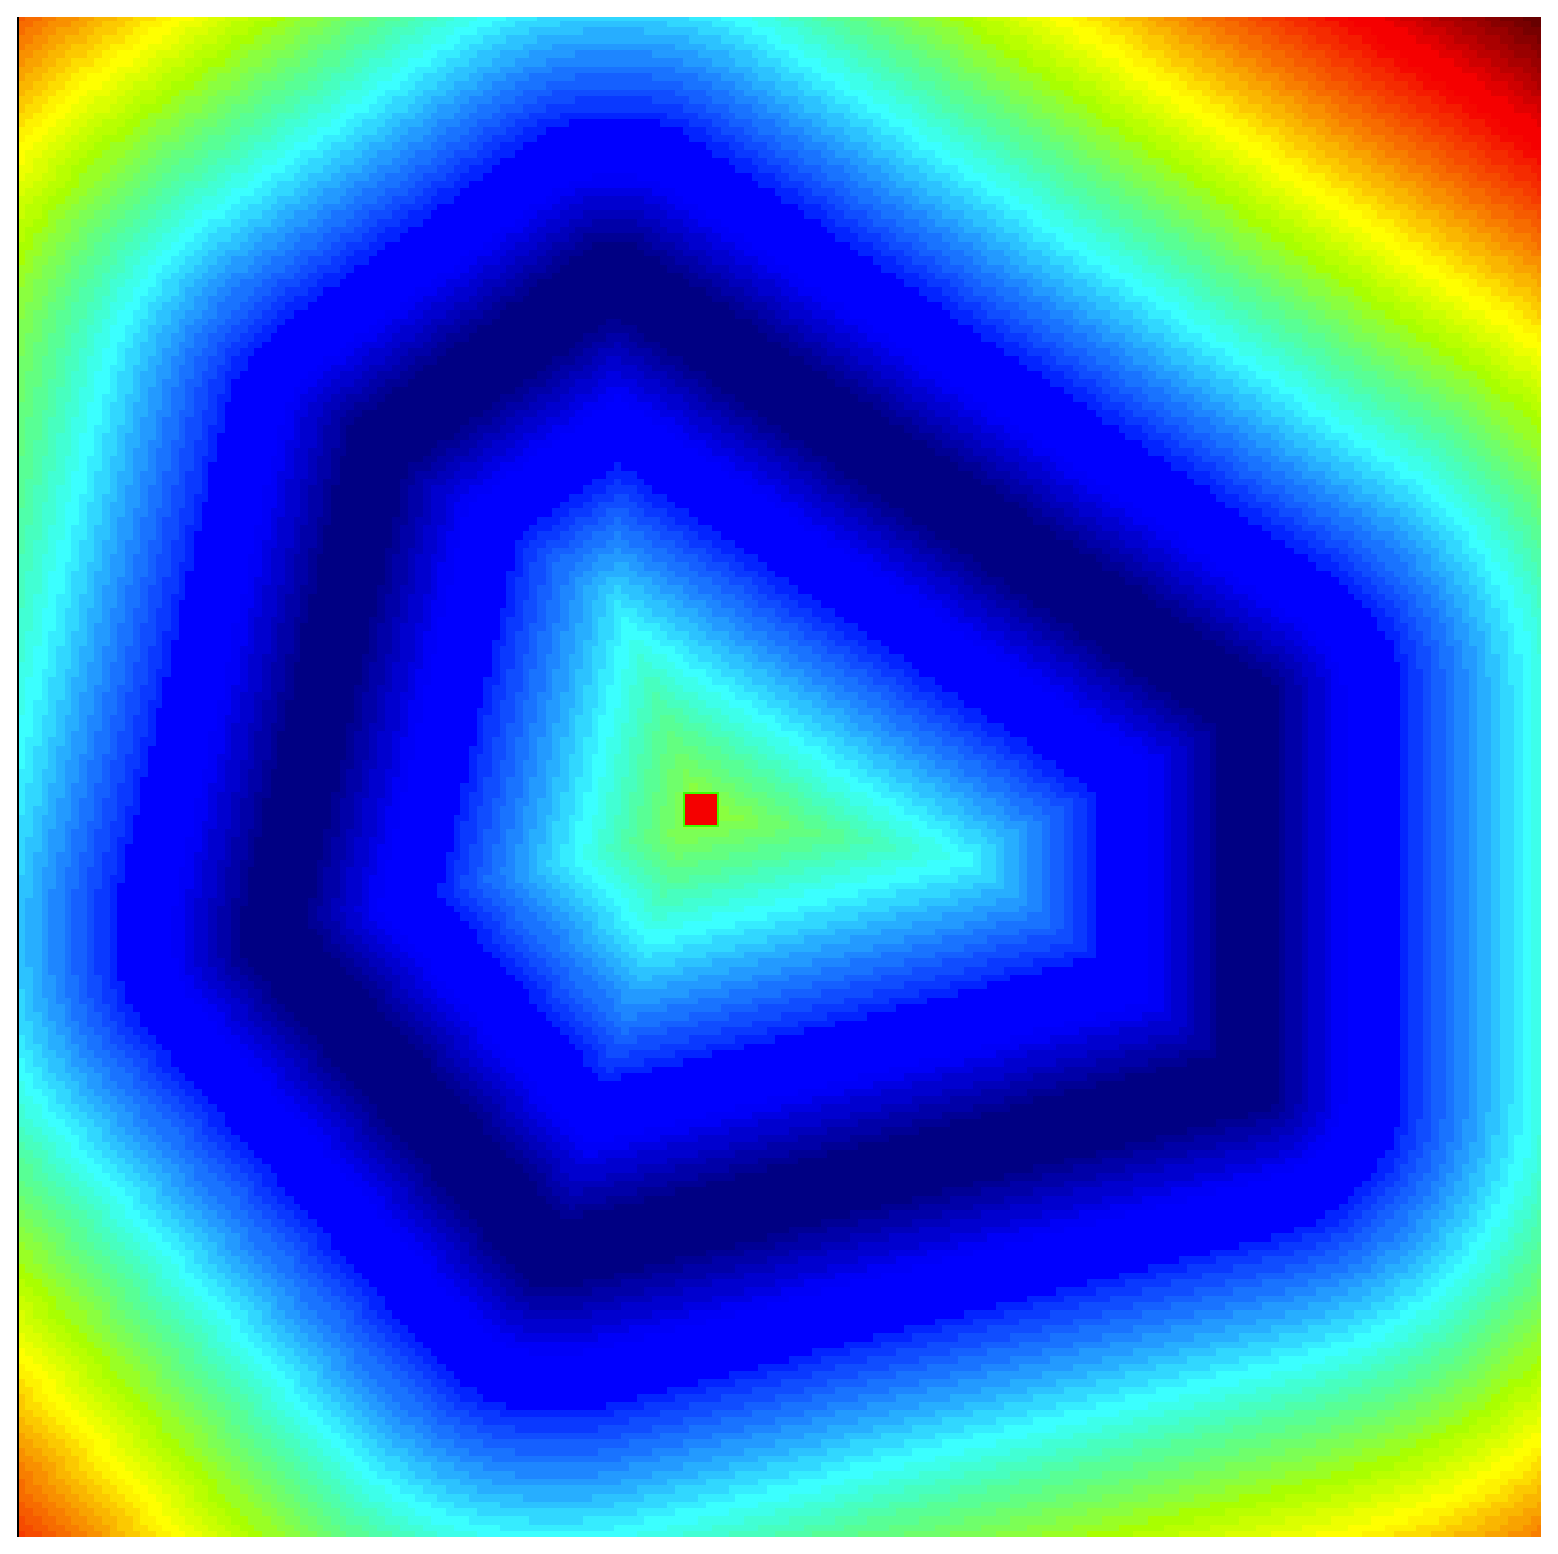
\includegraphics[width=0.33\textwidth, height=0.33\textwidth]{pictures/theoryCompleteCenter}\label{fig:theoryCompleteCenter}}\\
%
\subfloat[][]{
\includegraphics[width=0.33\textwidth, height=0.33\textwidth]{pictures/theoryIncomplete}\label{fig:theoryIncomplete}}
\subfloat[][]{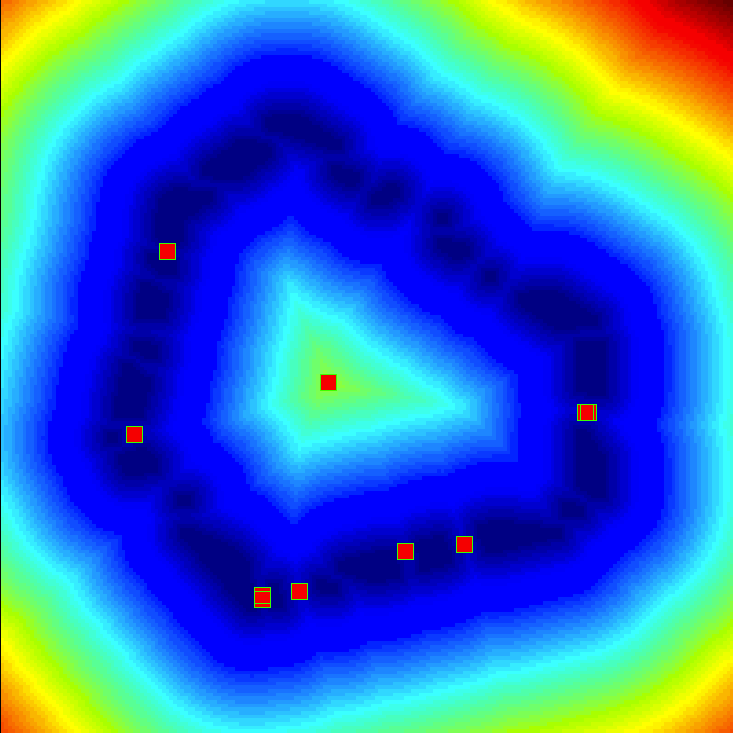
\includegraphics[width=0.33\textwidth, height=0.33\textwidth]{pictures/theoryIncompleteLocalMax}\label{fig:theoryIncompleteLocalMax}}
\subfloat[][]{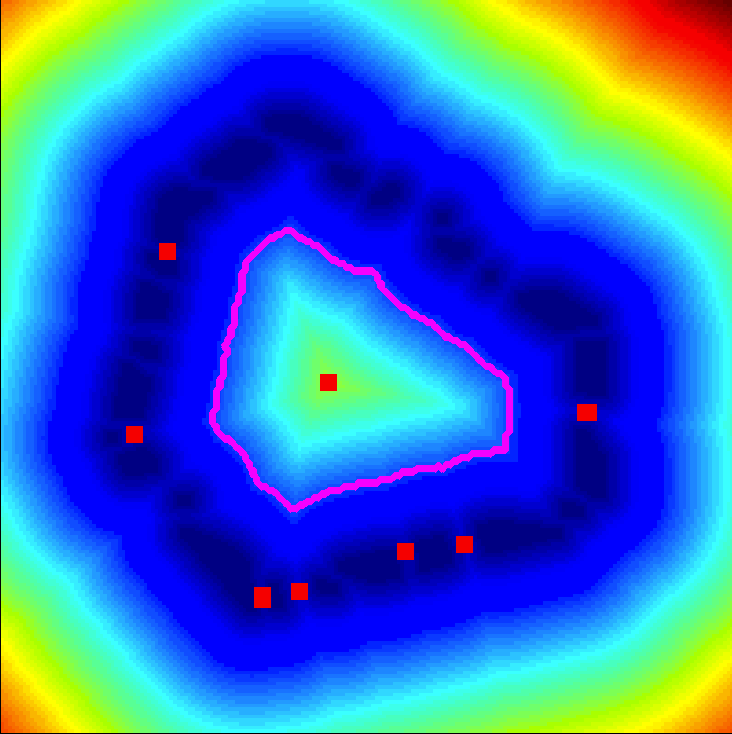
\includegraphics[width=0.33\textwidth, height=0.33\textwidth]{pictures/theoryIncompleteThreshold}\label{fig:theoryIncompleteThreshold}}\\
%
\subfloat[][]{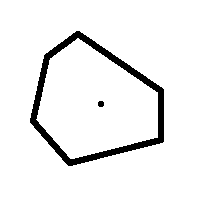
\includegraphics[width=0.33\textwidth, height=0.33\textwidth]{pictures/theoryNoise}\label{fig:theoryNoise}}
\subfloat[][]{\includegraphics[width=0.33\textwidth, height=0.33\textwidth]{pictures/theoryNoiseLocalMax}\label{fig:theoryNoiseLocalMax}}
\subfloat[][]{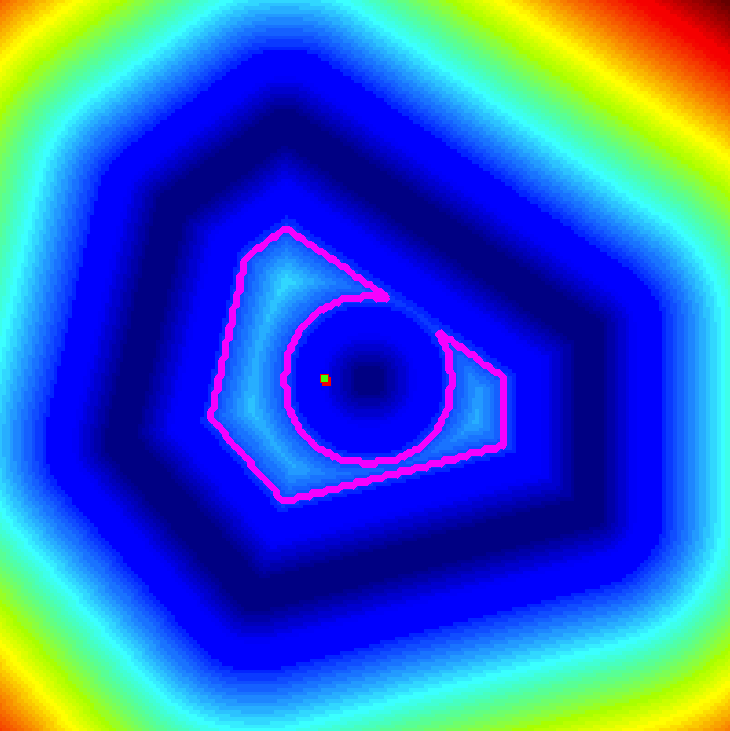
\includegraphics[width=0.33\textwidth, height=0.33\textwidth]{pictures/theoryNoiseCentroid}\label{fig:theoryNoiseCentroid}}
%
\caption{%
\subref{fig:theoryComplete}: complete synthetic cell membrane;
\subref{fig:theoryCompleteDistance}: distance map from~\subref{fig:theoryComplete};
\subref{fig:theoryCompleteCenter}: local maximum red square represents the local maxima of~\subref{fig:theoryCompleteDistance}.\\
%
\subref{fig:theoryIncomplete}:
 incomplete synthetic cell membrane;
\subref{fig:theoryIncompleteLocalMax}:
 distance map from~\subref{fig:theoryIncompleteLocalMax},
 the red squares are the local maximas;
\subref{fig:theoryIncompleteThreshold}: 
 thresold of~\subref{fig:theoryIncompleteLocalMax} 
 at 20pixels, represented by the magenta contour (approximation of the voronoi cell).
 Note that the only local maxima present in the
 thresholded area is the \emph{cell site}.\\
%
\subref{fig:theoryNoise}:
 noisy synthetic cell membrane;
\subref{fig:theoryNoiseLocalMax}:
 distance map from~\subref{fig:theoryNoise},
 the red squares are the local maximas;
\subref{fig:theoryNoiseCentroid}:
 threshold of~\subref{fig:theoryNoiseLocalMax} at 20pixels,
 represented by the magenta contour.
 Note that the centroid of the thresholded region (green square)
 is very close to the \emph{cell site} (red square).%
}
  \label{fig:incompleteMembraneSynthetic}
\end{figure}



\begin{figure}[htb]
  \centering
%
\subfloat[][]{\includegraphics[width=0.3\textwidth, height=0.3\textwidth]%
{pictures/propReconstructedMembrane}\label{fig:propReconstructedMembrane}}\hspace{3pt}
%
\subfloat[][]{\includegraphics[width=0.3\textwidth, height=0.3\textwidth]%
{pictures/propThresholdedReconstructed}\label{fig:propThresholdedReconstructed}}\hspace{3pt}
%
\subfloat[][]{\includegraphics[width=0.3\textwidth, height=0.3\textwidth]%
{pictures/propDistance}\label{fig:propDistance}}\\
%
%
%
%
%
%
\subfloat[][]{\includegraphics[width=0.3\textwidth, height=0.3\textwidth]%
{pictures/propNucleiMask}\label{fig:propNucleiMask}}\hspace{3pt}
%
\subfloat[][]{\includegraphics[width=0.3\textwidth, height=0.3\textwidth]%
{pictures/propDistThresh}\label{fig:propDistThresh}}\hspace{3pt}
%
\subfloat[][]{\includegraphics[width=0.3\textwidth, height=0.3\textwidth]%
{pictures/propDistThreshMask}\label{fig:propDistThreshMask}}\\
%
\subfloat[][]{\includegraphics[width=0.3\textwidth, height=0.3\textwidth]%
{pictures/propThresholdedDistanceMap}\label{fig:propThresholdedDistanceMap}}\hspace{3pt}
%
\subfloat[][]{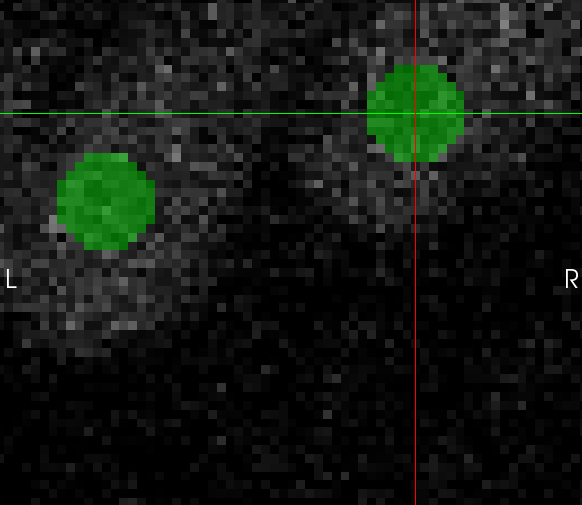
\includegraphics[width=0.3\textwidth, height=0.3\textwidth]{pictures/propCentroids}\label{fig:propCentroids}}\\
%
\caption{\\%
Figures \subref{fig:propReconstructedMembrane}, \subref{fig:propThresholdedReconstructed}, \subref{fig:propDistance}: Distance map creation from the reconstructed membrane data.\\
\subref{fig:propReconstructedMembrane}: Reconstructed membrane with\cite{kishoreMembrane};
\subref{fig:propThresholdedReconstructed}: Binary image of the membrane;
\subref{fig:propDistance}: Distance map created from the incomplete membrane data (red values are higher, and dark values are lower).\\
\\
%
%
Figures \subref{fig:propNucleiMask}, \subref{fig:propDistThresh}, \subref{fig:propDistThreshMask}, \subref{fig:propThresholdedDistanceMap}, \subref{fig:propCentroids}: Localisation of the \emph{sites} from the threshoded distance map and the thresholded nuclei channels:\\
\subref{fig:propNucleiMask}: Nuclei mask used for masking the approximate VRs;
\subref{fig:propDistThresh}: Thresholded distance map of the membrane : approximate VRs;
\subref{fig:propDistThreshMask}: Masked approximate VRs. Their \emph{centroid} is to the \emph{cell site}.
\subref{fig:propThresholdedDistanceMap}: Close up of two approximate VRs masked with the thresholded nuclei;
\subref{fig:propCentroids}: Nuclei detection (in green) corresponding to the \emph{centroids} of the masked approximate VRs of figure~\subref{fig:propThresholdedDistanceMap}.%
}
  \label{fig:propIllustr}
\end{figure}




\subsection{Difficulties and solutions}
\label{sect:difficultiesTheory}

\subsubsection{Profusion of local maximas}

As the membrane is a convex polygon, we should have only one local maxima per VR, 
and from that, determining the VS should be easy, but,
the lack of information on the membrane channel creates local maxima in the holes location (as illustrated figure~\ref{fig:theoryIncompleteLocalMax}).
If the holes in the membrane are much smaller than the cell's radius,
those unwanted local maximas will have much smaller value than the one in the middle of the cell,
because they will be close to the hole's boundary.
We use a simple threshold on the distance map to invalidate smaller local maximas, and keep the high values of the distance map (see figure~\ref{fig:theoryIncompleteThreshold}), this gives us a region inside the VR, that we name "approximate VR".
This region is inside the VR, and can be considered as an erosion of it. 

Another reason for having several local maximas, is noise in the membrane channel (as illustrated figure~\ref{fig:theoryNoise}).
If a point far from the boundary of the cell is considered as membrane, the distances will be computed from this point, leading to two local maximas in one cell, of lower value (see figure~\ref{fig:theoryNoiseLocalMax}). This modifies the shape of the approximate VR, and the position of its center of mass.
If the noise is restricted to few points in the membrane, then we are able to recover the VS by computing the center of mass of the thresholded distance map (see figure~\ref{fig:theoryNoise}, \subref{fig:theoryNoiseLocalMax}, \subref{fig:theoryNoiseCentroid}).

\subsubsection{Shape of cell membranes}

In order to find an eroded approximation of the Voronoi cell, we use a simple thresholding on the distance map generated from the membrane.
Then, we locate the centroid of this region, but it happens that cells are not convex polygons, and in this case, the centroid can be outside the membrane (especially in bean shaped cells).
In order to keep the centroid inside the cell boundaries, we mask the Voronoi approximation, by the binarized nuclei channel.
Thus, our regions are restricted to parts of the image where a nuclei is present, and the centroid of the masked approximate Voronoi cell is located inside the nuclei.

\subsubsection{Membrane reconstruction}

As the membrane information is very poor, we use, a reconstruction method designed by Dr Kishore Mosaliganti {\etal}~\cite{kishoreMembrane}. This method is inspired by~\cite{tasdizen2005enhancement}, who presents a method for cell boundaries enhancement in 2D.
These methods are inspired by vessel enhancement techniques~\cite{frangi1998multiscale, manniesing2006vessel}.
The vessel enhancement algorithms' assumption is that vessel are constituted by succession of cylinders. Kishore's assumption is that membrane is constituted by plans.
Kishore's algorithm diffuses intensities along planar structures, instead of cylinders.

This method provides a very good denoising, but big holes in the membrane channel are still presents. In order to fill those holes and get a reconstructed membrane, Kishore uses a tensor voting reconstruction method~\cite{tensorvoting}.



%%%%%%%%%%%%%%%%%%%%%%%%%%%%%%%%%%%%%%%%%%%%%%%%%%%%%%%%%%%%%%%%%%%%%%%%%%%%%%%
%%%%%%%%%%%%%%%%%%%%%%%%%%%%%%%%%%%%%%%%%%%%%%%%%%%%%%%%%%%%%%%%%%%%%%%%%%%%%%%
%%%%%%%%%%%%%%%%%%%%%%%%%%%%%%%%%%%%%%%%%%%%%%%%%%%%%%%%%%%%%%%%%%%%%%%%%%%%%%%


\section*{Conclusion}

We present here a new method for detecting cell nuclei in noisy and incomplete 2 photon/confocal 3D datasets.
This method uses a simple assumption, and we proved that it is robust to loss of continuity in the membrane channel, and noise.
We described the theory, and explained the methodology, we will evaluate this method against existing algorithms to finally conclude about our contribution.






\chapter{Results}
\label{chapt:results}

We will evaluate three algorithms in this section:
the algorithm that was used when I arrived in the Megason Lab (see subsection~\ref{sect:megasonExisting}),
the variant of the Laplacian of Gaussian presented in \cite{al2009improved} : scale constrained Laplacian of Gaussian (see subsection~\ref{sect:farsight}),
and our proposed algorithm (see chapter~\ref{chapt:proposal}).



%%%%%%%%%%%%%%%%%%%%%%%%%%%%%%%%%%%%%%%%%%%%%%%%%%%%%%%%%%%%%%%%%%%%%%%%%%%%%%%
%%%%%%%%%%%%%%%%%%%%%%%%%%%%%%%%%%%%%%%%%%%%%%%%%%%%%%%%%%%%%%%%%%%%%%%%%%%%%%%
%%%%%%%%%%%%%%%%%%%%%%%%%%%%%%%%%%%%%%%%%%%%%%%%%%%%%%%%%%%%%%%%%%%%%%%%%%%%%%%



\section{Evaluation framework}

The evaluation is performed both on synthetic and real data. We provide information about the detection quality, the robustness, and the processing time of each algorithm.

\subsection{Evaluation data}

The data presented in this section is illustrated in the annex~\ref{annex:EvalData}.

\subsubsection{Synthetic data}

Synthetic data was provided for evaluating the robustness of algorithms.
The data set consists into 10 3D images containing noisy nuclei and membrane channels.
The datasets are non isotropic, and the resolution along z is 5 times the resolution along x and y.
The amount of nuclei goes from 100 to 1000, with increasing level of noise.

This dataset is very useful for testing robustness to noise and anisotropy, but it does not include stacked nuclei.


\subsubsection{Real data}

\begin{figure}[htb]
\begin{center}
\leavevmode
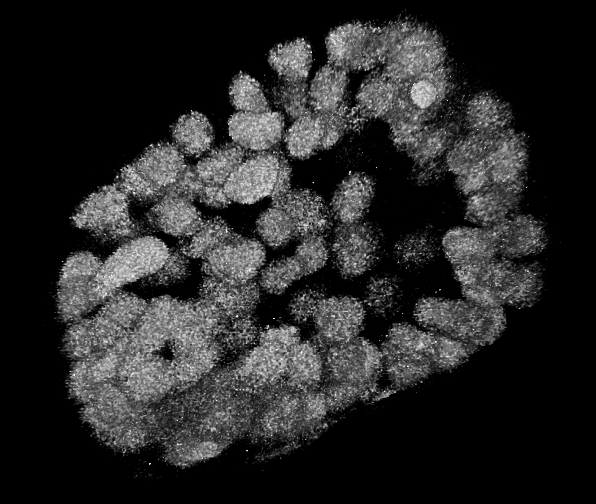
\includegraphics[width=0.6\textwidth]{pictures/rawRaycast}
\end{center}
\caption{3D rendering by ray tracing of the nuclei channel of the real dataset used for evaluation.}
\label{fig:rawRaycast}
\end{figure}

The real data corresponds to 3D dataset of the ear of a zebrafish embryo (see figure~\ref{fig:rawRaycast}).
It consists in a membrane and nuclei channel, and a manual segmentation of nuclei in a region of the image.
There are 141 nuclei in the manually segmented region of the dataset. 

\subsection{Evaluation criterion}

We evaluate:
\begin{itemize}
\item the number of correctly detected nuclei, which correspond to one detection in a manually segmented nuclei,
\item the number of outside detections corresponding to detections of nuclei outside of manually segmented nuclei.
\item the number of over-detection corresponding to re-detection of an already detected nuclei (two or more detections inside a cell nuclei).
\item "success" which corresponds to:\\
 \[
 \frac{correctly detected}{undetected + over detected + outside detections + correctly detected} 
 \]
\end{itemize} 

We also evaluate the processing time of the algorithms using information provided by the unix 'time' command, as it is able to give the time spent by each cpu on the processing task, making the implementation less determinant for the evaluation.


%%%%%%%%%%%%%%%%%%%%%%%%%%%%%%%%%%%%%%%%%%%%%%%%%%%%%%%%%%%%%%%%%%%%%%%%%%%%%%%
%%%%%%%%%%%%%%%%%%%%%%%%%%%%%%%%%%%%%%%%%%%%%%%%%%%%%%%%%%%%%%%%%%%%%%%%%%%%%%%
%%%%%%%%%%%%%%%%%%%%%%%%%%%%%%%%%%%%%%%%%%%%%%%%%%%%%%%%%%%%%%%%%%%%%%%%%%%%%%%


\section{Evaluation results}


\subsection{Evaluation on synthetic data}

The evaluation results are detailed in annex~ref{annex:Eval}. We present here the "success" percentage of the algorithms (see tabular~\ref{tab:simuSuccess}).
\begin{figure}[htb]
\begin{center}
\subfloat[][]{
\begin{tabular}{|l|l|}
\hline Algorithm & Success (\%) \\ 
\hline Existing algorithm in Megason Lab & 40 \\ 
\hline Scale constrained Laplacian of Gaussian & 98 \\ 
\hline Proposal & 99 \\ 
\hline
\end{tabular}\label{tab:meanSuccess}}\\
%
\subfloat[][]{
\begin{tabular}{|l|l|}
\hline Algorithm & Success (\%) \\ 
\hline Existing algorithm in Megason Lab & 7 \\ 
\hline Scale constrained Laplacian of Gaussian &  93 \\ 
\hline Proposal & 95 \\ 
\hline
\end{tabular}\label{tab:hardSuccess}}
\end{center}
\caption{Evaluation of 3 algorithms on 10 synthetic datasets of increasing difficulty:\\
\subref{tab:meanSuccess} presents the mean value of "success" over the 10 synthetic datasets containing 100 to 1000 cells.
\subref{tab:hardSuccess} presents the "success" on the hardest dataset, very noisy and containing 1000 cells.
}
\label{tab:simuSuccess}
\end{figure}
The evaluation on synthetic data proved the proposed algorithm to have the highest "success" percentage,
meaning that it detects more nuclei without mistakes. Then comes the scale constrained Laplacian of Gaussian which is very robust
but has more detections outside of nuclei than the proposed algorithm. Finally the existing algorithm performs worse than the two others,
after a certain amount of noise in the images.


\subsubsection{Evaluation a segmented dataset}

We present here the results of the evaluation on a real 2-photon/confocal dataset (see tabular~\ref{tab:realEval}). We can see that all algorithm preforms poorly on this dataset.
The difficulties mentioned in section~\ref{setc:ChallengesData}, makes this dataset very hard to process. Another difficulty is the particular shape of the cells in this region: they are elongated, and nuclei are most of times located next to the border of the cells.
This evaluation let us compare the three algorithms on a very hard dataset.
\begin{figure}[htb]
\begin{center}
\begin{tabular}{|p{2.5cm}|l|l|p{1.3cm}|l|}
\hline Algorithm & Correct (\%) & Outside (\%) & Over-detected (\%) & Success (\%) \\ 
\hline Existing algorithm in Megason Lab & 50 & 40 & 26 & 30 \\ 
\hline Scale constrained Laplacian of Gaussian &  74 & 36 & 6 & 51 \\ 
\hline Proposal & 60 & 21 & 2 & 49 \\
\hline
\end{tabular}
\end{center}
\caption{Evaluation of 3 algorithms on a real dataset of the ear of a zebrafish embryo. the results are normalized by the number of cells in the image.}
\label{tab:realEval}
\end{figure}

We can see that the scale constrained Laplacian of Gaussian outperforms both existing and presented algorithms in terms of detected cells.
It is also important to notice that it make more outside of nuclei and over-detections than the proposed algorithm.
The existing algorithm performs worse than the two others.


\subsection{Time evaluation}

We computed the execution time of the three algorithms, on the real dataset (see tabular~\ref{tab:timeEval}
\begin{figure}[htb]
\begin{center}
\begin{tabular}{|l|l|}
\hline Algorithm & Processing time (min) \\ 
\hline Existing algorithm in Megason Lab & 16 \\ 
\hline Scale constrained Laplacian of Gaussian &  22 \\ 
\hline Proposal & 21 \\
\hline
\end{tabular}
\end{center}
\caption{Processing time of 3 algorithms on a real dataset of 1024x1024x57 voxels. Inputs are raw nuclei and membrane channels.}
\label{tab:timeEval}
\end{figure}
The fastest algorithm is the one currently used in the Megason lab, with an execution time of 16 minutes.
Then the Laplacian of Gaussian and the Proposal have approximatively the same processing time.
We decided to focus on algorithms rather than implementation,
so the given times are the sum of the time spent by each processor,
thus, we don't advantage too much the multi-threaded implementations. 



%%%%%%%%%%%%%%%%%%%%%%%%%%%%%%%%%%%%%%%%%%%%%%%%%%%%%%%%%%%%%%%%%%%%%%%%%%%%%%%
%%%%%%%%%%%%%%%%%%%%%%%%%%%%%%%%%%%%%%%%%%%%%%%%%%%%%%%%%%%%%%%%%%%%%%%%%%%%%%%
%%%%%%%%%%%%%%%%%%%%%%%%%%%%%%%%%%%%%%%%%%%%%%%%%%%%%%%%%%%%%%%%%%%%%%%%%%%%%%%


\section{Implementation details}

The data we are processing are 3D plus time, this represents huge datasets, that are hardly processed by Matlab.
Thus, prototyping was done in {\C++}, using medical image processing libraries such as the Insight ToolKit (ITK)
or the Visualization ToolKit (VTK).

\subsection{Programmation language and libraries}

The algorithms developed in the Megason lab are directly used by Biologists on a day to day basis.
They are integrated to the program developed by a group of computer scientists (Arnaud Gelas, Lydie Souhait and Nicolas Rannou): {\gofigure}.
This program is exclusively coded in \C++ and integrates ITK and VTK.
Our algorithm must be coded in such way that this group can reuse them and integrate them (abundant documentation and accessibility to source code).

The use of ITK give us the opportunity to develop fast algorithms, able to process huge datasets, but it also adds a lot of complexity to the prototyping process.


\subsection{Reproducibility}

All developed algorithms but Kishore's are open source and distributed on the internet, on \href{http://github.com/antonin07130}{Github}.
This provides other computer scientists with the opportunity to download and compile the programs I created.
Those are open source and cross platform. The proposed algorithm consists in a series of small programs linked by a bash script.


%%%%%%%%%%%%%%%%%%%%%%%%%%%%%%%%%%%%%%%%%%%%%%%%%%%%%%%%%%%%%%%%%%%%%%%%%%%%%%%
%%%%%%%%%%%%%%%%%%%%%%%%%%%%%%%%%%%%%%%%%%%%%%%%%%%%%%%%%%%%%%%%%%%%%%%%%%%%%%%
%%%%%%%%%%%%%%%%%%%%%%%%%%%%%%%%%%%%%%%%%%%%%%%%%%%%%%%%%%%%%%%%%%%%%%%%%%%%%%%

\section{Conclusion}

We can see that the proposed algorithm, processing mainly the membrane information, outperforms the existing algorithm in the Megason Lab.
The scale constrained Laplacian of Gaussian performs better than those two algorithms for detecting seeds, but also produces more false detections
(over detections and out of nuclei detections).
It is important to notice that the real dataset is a special arrangement of cells, and it would be important to test the algorithms on a different dataset. Also, this dataset has been masked by a "region of interest", in such way that all membranes facing outer parts of the region were left open leading to detection of nuclei out of the region of interest.
It is also hard to compare those results directly with those of articles which evaluate their algorithms after the segmentation, as most of them use a segmentation refinement step,
for eliminating objects that are segmented but do not correspond to nuclei in terms of shape characteristics.
A visual comparison showed us that in case of stacked nuclei, our proposal was able to correctly separate nuclei when the two other algorithm would fail. It is unfortunately hard to display such results\footnote{
I created two applications for this purpose that can be found on Github:
\begin{description}
\item[\href{http://github.com/antonin07130/itkCompareProject}{Compare Project}]: which is useful for comparing two itk images slice by slice, especially "compareguiexample" which provides a GUI for visualizing and comparing such datasets.
\item[\href{http://github.com/antonin07130/SeedVisu}{SeedsVisualization}]: which takes a list of point and an itk 3D dataset as inputs. This programs renders the volume with a ray tracing algorithm, and superpose the points listed in the text file.
\end{description}
} in a paper format, as data are three dimensional and results are points within these datasets.




\chapter{Conclusion}
%%5- Partial conclusion.
%%    1- What is new?
%%    2- Did you improve existing methods? in which way?
%%        if not, why?
%%    3- Future work.

First, we will talk about our contribution, the future work that can be done, to finally open the report to my future works in research.

%
%While in the Megason Lab, I have been working on segmenting fluorescent microscopy images.
%Datas are four-dimensional (space and time), and represent regions (ear, brain...) of a developing zebrafish.
%
%
%The creation of this model is a thesis subject : cells lineage registration in microscopy, during which I would like to extend my work.
%
%Prior to arriving in the laboratory, I have been working on cell membrane. I have then concentrated my researches on cell nuclei detection and localization.




\section{Our contribution}

We proposed a new algorithm capable of performing well in noisy 2 photons/confocal 3D datasets.
Most of current methods are based on gradient information on the nuclei channel, but this channel is often very noisy, and this information hard to retrieve.
The proposed method makes use of the membrane channel as the main source of information,
and provides is able to detect nuclei where gradient based\cite{al2009improved} algorithms fail. 
This algorithm was compared to two other recent methods and proved to provide better results than the one currently used in the Megason lab.


\section{Improvements of actual method}

The proposed method outperforms the method currently used in the megason lab by 18 points
(see tabular~\ref{tab:realEval}), according to our "success" measure, representing the amount of correctly placed detections.
We also proved it to be more robust to noise in the synthetic datasets.
We plan to use a fusion framework, later on, to fuse the results from this method, and from the scale constrained LoG. Using information of different algorithm depending on the region ( our mehtod outperforms the scale constrained LoG in case of stacked nuclei).


\section{Future work}


\subsection{Cell detection proposal}

There are lots of track to improve the cell detection algorithm:
\begin{itemize}
  \item  We can fuse information from this algorithm, and the scale constrained LoG, in order to correctly separate nuclei in area where they are stacked.
  \item We can automate the thresholding of the membrane distance map, to get the approximate Voronoi cells, with a clustering algorithm based on values of the local maximas of the distance map: there should be a cluster of local maximas under the threshold level corresponding to holes in the membrane, and a cluster of local maximas above the threshold corresponding to local maximas inside the Voronoi cell.
  \item  We can also automate the choice of the thresholds for nuclei and membrane binary masks, based on histograms of denoised images.
  \item  We can also use non linear resampling methods, for improving the resolution among z.
  \item  We could combine the results of several algorithms  : use our proposal in regions where nuclei are clumped, 
  and the contour based algorithms (Kishore's or the improved Multiscale Laplacian of Gaussian) in region where nuclei are isolated.
  The detection of such regions can be done by analysing the size of the connected components of the binarized nuclei image:
  clumped nuclei correspond to large connected components. For the purpose of nearest neighbour research, a Kdtree can be used.
\end{itemize}


\subsection{Cell membrane reconstruction and segmentation}

Once we have a good enough seed detection, we can use this information, to reconstruct the membrane channel based.
Indeed, we can use the center of the nuclei and consider the membrane as a Voronoi diagram which sites are the nuclei's centres.
With the help from this information, membrane reconstruction can be carried out.

We also have points within each cell; this crucial information will be very helpful for initializing level set approaches for segmenting both nuclei and cell membrane.
Knowing what the topology of the membrane is is an information
that a topology constrained local level set could use (\cite{han2003topology,lankton2008localizing}), and we are working on developing such algorithm.


\section{Personal conclusion}

I have had an amazing opportunity, during this thesis,
to discover and participate to the American research.
I was able to get in touch with worldwide recognized
image processing scientists during the NA-MIC\footnote{
The National Alliance for Medical Image Computing (NA-MIC) is a multi-institutional, interdisciplinary team of computer scientists, software engineers, and medical investigators who develop computational tools for the analysis and visualization of medical image data.}
summer project week in MIT, and to work in a collaborative environment.

The master thesis in the Megason lab taught me a lot, not only about the research environment, but also about hardcore programming techniques that provided me with a good understanding of extremely powerfull \C++ libraries. I am now able to efficiently program using ITK and VTK, and thus can work on huge dataset, and reuse the numerous image processing filters already implemented by medical image scientists.

\section{Future}

The current project is part of a long term project which is registration of cell lineages in Microscopy.
Indeed, in order to be able to track cells in space and time, biologists image living specimen. Then, we have to automatically detect and segment the plethora of cells of the organism. That is what I have been working on during my master thesis.
Once we will be able to correctly detect and segment the cells and the nuclei, we will have to find ways to track cells across time. And finally, once we got the cell lineages of the whole organism, we will have to find ways to compare different specimens. That is the challenging subject I will be working on the next three years, for my phd thesis, in collaboration with the Creatis laboratory and the Megason Laboratory.


%\subsubsection{Implementation}
%After reading and understanding the article, I checked out the code from the Farsight Toolkit. The code has been developed two years ago and is not maintained any more.
%There was few documentation and comments, and the use of global variables made it hard to understand.
%I decided to start from scratch and reimplement the algorithm.
%

%The idea was to reimplement only the part of the algorithm of \cite{al2009improved} concerning the cell nuclei detection.
%The goal being to improve our initialization of the watershed algorithm. I was able to work with Raghav K. Padmanabhan, from the Roysam lab (who develops FTK),
%during the NA-MIC\footnote{The National Alliance for Medical Image Computing (NA-MIC) is a multi-institutional, interdisciplinary team of computer scientists,
%software engineers, and medical investigators who develop computational tools for the analysis and visualization of medical image data.} summer project week, in MIT.
%We tried to apply the FTK nuclei detection technique to 3D datasets, and to extract the Scale-constrained Laplacian of Gaussian implementation from the source code.
%
%A visual comparison of the binarization proceed by Kishore's algorithm and by the Farsight ToolKit led to the conclusion that Kishore's binarization
%was proceeding longer, but providing smoother results, which are important for the distance map step. That's the reason why, for the comparison of both algorithm,
%I reimplemented the Scale Constrained Laplacian of Gaussian and integrated it to Kishore's processing pipeline.
%
%




%
%
%
%\chapter{Conclusion du PFE}
%
%
%\section{Conclusion de la partie ingénierie}
%
%Durant ce PFE, j'ai travaillé sur des projets très variés.
%Ces projets étaient motivés par des objectifs scientifiques et nécessitaient chacun un haut niveau de technicité.
%
%J'ai eu l'occasion d'apprendre énormément,
%notamment dans le domaine des sciences informatiques,
%et du traitement de l'image.
%
%J'ai aussi découvert le milieu de la recherche, dont l'organisation est
%totalement différente de celle du milieu industriel.
%La hiérarchie, et les intérêts de chaque scientifique sont moins apparents que dans une entreprise et ce PFE a été riche en enseignements sur ce plan.
%Je suis parvenu à très bien m'intégrer dans l'équipe du Megason Lab en général,
%et à établir de bonnes relations de travail avec les divers scientifiques
%impliqués dans les projets sur lesquels j'ai travaillé.
%
%Cela m'a permis d'acquérir une base solide pour mener des recherches dans ce domaine.
%Après une importante phase d'apprentissage, je maitrise maintenant des librairies de renom
%(ITK, VTK,Qt), les systèmes unix, et la gestion de versions.
%
%J'ai pu aussi établir des contacts dans la communauté
%des traiteurs d'image par le biais de collaborations
%(Matthiew MacCormick), ou de d'"ateliers" (workshops) internationaux
%(participation à la NAMIC
%\footnote{La National Alliance for Medical Image Computing (NAMIC), est un réseau de professionnels de traitement d'images médicales. Ce réseau organise des conférences et des ateliers de travail ("workshop"), durant lesquels les scientifiques peuvent collaborer.}
%summer project week, au Massachusetts Institute of Technologies).
%
%
%\section{Projet professionnel}
%
%Ce PFE s'inscrit dans un projet professionnel construit durant ma scolarité à l'INSA de Lyon.
%Mon inscription à l'INSA de Lyon a été grandement motivée par l'ouverture de l'école à l'international. J'ai ainsi effectue mon stage ouvrier en Afrique du Sud. Profitant d'une première expérience professionnelle à l'international.
%
%Lors de ma seconde année a l'INSA de Lyon, j'ai choisi l'option SCiences et ANglais (SCAN).
%Cette filière regroupe les élèves ayant un niveau suffisant pour pouvoir suivre la formation généraliste en anglais.
%Elle s'accompagne d'une bourse pour un bref séjour linguistique dans une université étrangère.
%J'ai profité de ce financement pour aller au Trinity College en Irlande où
%j'ai pu avoir ma première expérience académique à l'étranger.
%
%J'ai ensuite choisi le département
%Génie Électrique qui permet de bénéficier d'un grand panel de compétences,
%notamment dans des domaines rattachés à l'électronique et l'informatique.
%
%
%Continuant l'expérience internationale, j'ai effectué mon stage industriel au
%Fraunhofer Institute, Center for Manufacturing Innovation, aux États Unis.
%J'ai été impliqué dans un projet de grande ampleur, financé par le département de la défense américain.
%Ce stage m'a énormément apporté en plus de l'expérience technique : il s'agissait d'une immersion dans la culture américaine, et j'ai eu une première expérience managériale en dirigeant une équipe d'ouvriers.
%C'est après ce stage que j'ai passé le test TOEIC validant un très bon niveau d'expression et de compréhension en anglais,
%avec un score de neuf cent quatre-vingt sur neuf cent quatre-vingt dix.
%
%
%Le PFE au Megason Lab possède des attraits indéniables :
%il s'agit d'un stage de recherche perfectionnant mes connaissances en traitement de l'image.
%Il s'agit aussi d'une expérience internationale dans une université renommée : Harvard Medical School.
%Ainsi, en plus de prendre plaisir à travailler en recherche, j'ouvre la porte à de nombreuses opportunités professionnelles.
%
%Comme je suis intéressé par les domaines techniques,
%je compte profiter de l'opportunité de poursuivre mes études pour obtenir un doctorat en mathématiques appliquées,
%au cours d'une thèse élaborée en collaboration avec le laboratoire CREATIS (INSA Lyon)
%et le laboratoire Megason (Harvard Medical School).
%Je passerai ainsi la moitié de mon temps en France, et l'autre moitié aux États Unis.
%En plus de pouvoir travailler sur un domaine passionnant,
%je pourrai ainsi bénéficier d'une équivalence avec un PhD (diplôme très reconnu à l'international). 
%
%Je compte ensuite mettre en valeur ma capacité a travailler dans un contexte international,
%dans des domaine à haute technicité pour trouver un emploi  dans le secteur privé.
%Je pourrai mettre en avant mes capacités en traitement du signal pour travailler dans le médical ou l'aéronautique.
%
%Mon ambition à long terme est de migrer vers des responsabilités managériales après avoir une très bonne maitrise de la technique.

\chapter*{Thanks}
\phantomsection
\addcontentsline{toc}{chapter}{Thanks}

I would like to thank, for their help and participation to my thesis, the following persons.

\begin{center}
Sean MEGASON\\
Kishore MOSALIGANTI\\
Arnaud GELAS\\
Olivier BERNARD\\
Rémy PROST\\
Matthiew MACCORMICK\\
Isabelle BLOCH\\
Nicolas RANNOU\\
Lydie SOUHAIT\\
Amelia GREEN\\
Nikolaus OBHOLZER\\
Ramil NOCHE\\
Raghav K. PADMANABHAN\\
Luis IBANEZ\\
\end{center}

And also the teams in Creatis LRMN, and in the Megason lab, for the great working ambiance I could find in these laboratories.

\appendix







%%%%%%%%%%%%%%%%%%%%%%%%%%%%%%%%%%%%%%%%%%%%%%%%%%%%%%%%%%%%%%%%%%%%%%%%%%%%%%%
%%%%%%%%%%%%%%%%%%%%%%%%%%%%%%%%%%%%%%%%%%%%%%%%%%%%%%%%%%%%%%%%%%%%%%%%%%%%%%%
%%%%%%%%%%%%%%%%%%%%%%%%%%%%%%%%%%%%%%%%%%%%%%%%%%%%%%%%%%%%%%%%%%%%%%%%%%%%%%%

\chapter{The team of the Megason lab}

The Megason Lab's employee are post-doc researchers. Two domains of expertise are present : Biology and informatics.
The biology team leads researches on the development of zebra fishes,
and the computer team works on developing a program for visualization, segmentation, and tracking of cells adapted to microscopy data.

{\small \begin{tabular*}{1.0\textwidth}{@{\extracolsep{\fill}}|p{2.5cm}| p{3.cm}|p{3.5cm}|c|}
\hline Name & Status & Interest & Nationality \\ 
\hline Sean Megason & Professor & Financing and managing the laboratory. & USA \\ 
\hline Ramil Noche & Post-doctoral fellow & dynamics and function of gene regulatory networks. & Philipines \\ 
\hline Fengzhu Xiong & Graduate student & cell differentiation mechanism to create neurons and skin cell. & Chine \\ 
\hline Nikolaus Obholzer & Post-doctoral fellow  & Ear development and regeneration. &  Allemange \\ 
\hline Paul Cowgill & Graduate student & Synthetic biology, noise and development. & USA \\ 
\hline David Tulga & Graduate student & Cellular development. &  USA \\ 
\hline Ian Swiburne & Post-doctoral fellow & Ear development. & USA \\ 
\hline Andrea Tentner & Post-doctoral fellow  & Cell differentiation in spinal cord. & USA \\ 
\hline Amelia Green & Post-doctoral fellow  & Variation and regulation in organ development. & Angleterre \\ 
\hline Evan Schwab & Associate & Locations of genes responsible for mutations in the zebra fish ear using computational algorithm. & USA \\ 
\hline Dante D'India & Technicien & Animal care. & USA \\ 
\hline Arnaud Gelas & Research Engineer (senior) &  Developing {\gofigure}: Project management. &  France \\
\hline Kishore Mosaliganti & Post-doctoral fellow  & Image processing algorithms, registration and segmentation. & India \\ 
\hline Lydie Souhait & Research Engineer & Developing {\gofigure}: Responsible of the database (design, connexion, requests), and GUI & France \\
\hline Nicolas Rannou & Research Engineer &  Developing {\gofigure}: Responsible of the visualization in {\gofigure} & France \\
\hline Antonin Perrrot-Audet & Intern& Image processing : cells detection; developing {\gofigure} & France \\
\hline 
\end{tabular*} }




%%%%%%%%%%%%%%%%%%%%%%%%%%%%%%%%%%%%%%%%%%%%%%%%%%%%%%%%%%%%%%%%%%%%%%%%%%%%%%%
%%%%%%%%%%%%%%%%%%%%%%%%%%%%%%%%%%%%%%%%%%%%%%%%%%%%%%%%%%%%%%%%%%%%%%%%%%%%%%%
%%%%%%%%%%%%%%%%%%%%%%%%%%%%%%%%%%%%%%%%%%%%%%%%%%%%%%%%%%%%%%%%%%%%%%%%%%%%%%%




\chapter{Evaluation Data Illustrations}
\label{annex:EvalData}

\section{Real}

\begin{figure}[htb]
  \centering
%
\subfloat[][]{\includegraphics[width=0.3\textwidth, height=0.3\textwidth]%
{pictures/reelNucxy}\label{fig:reelNucxy}}\hspace{3pt}
%
\subfloat[][]{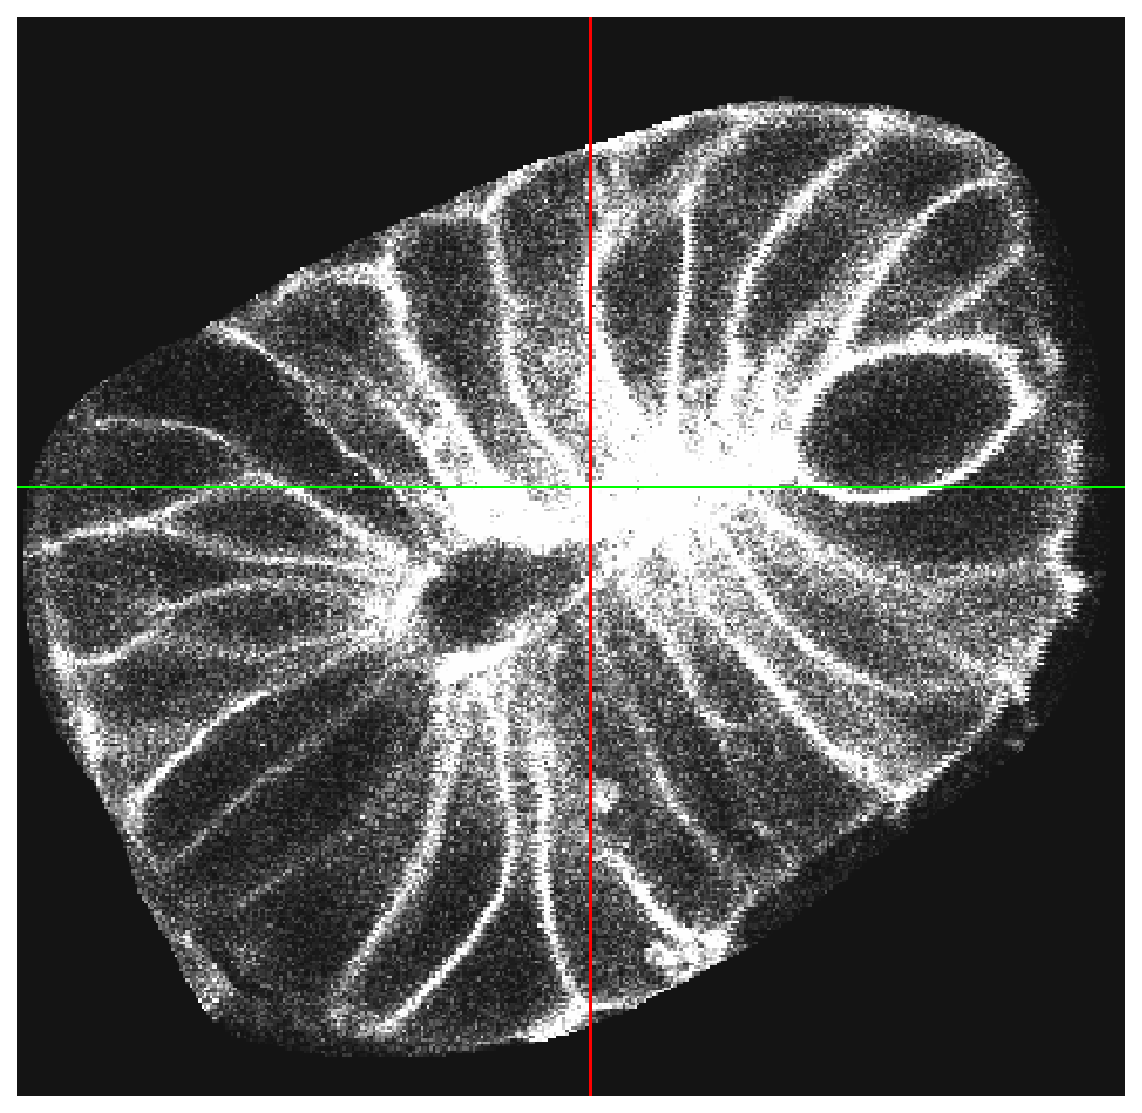
\includegraphics[width=0.3\textwidth, height=0.3\textwidth]
{pictures/reelMembxy}\label{fig:reelMembxy}}\\
%
\subfloat[][]{\includegraphics[width=0.3\textwidth, height=0.3\textwidth]%
{pictures/reelNucxz}\label{fig:reelNucxz}}\hspace{3pt}
%
\subfloat[][]{\includegraphics[width=0.3\textwidth, height=0.3\textwidth]%
{pictures/reelMembxz}\label{fig:reelMembxz}}\hspace{3pt}
%
%
%
%
%
\caption{%
xy (\subref{fig:reelNucxy},\subref{fig:reelMembxy})
 and yz (\subref{fig:reelNucxz}, \subref{fig:reelMembxz}) nuclei and corresponding membrane slices of the real dataset containing 141 cells.
}
  \label{fig:realData}
\end{figure}

\section{Synthetic}

\begin{figure}[htb]
  \centering
%
\subfloat[][]{\includegraphics[width=0.3\textwidth, height=0.3\textwidth]%
{pictures/validNuc1xy}\label{fig:validNuc1xy}}\hspace{3pt}
%
\subfloat[][]{\includegraphics[width=0.3\textwidth, height=0.3\textwidth]%
{pictures/validMemb1xy}\label{fig:validMemb1xy}}\\
%
\subfloat[][]{\includegraphics[width=0.3\textwidth, height=0.3\textwidth]%
{pictures/validNuc1yz}\label{fig:validNuc1yz}}\hspace{3pt}
%
\subfloat[][]{\includegraphics[width=0.3\textwidth, height=0.3\textwidth]%
{pictures/validMemb1yz}\label{fig:validMemb1yz}}\\
%
%
%
\subfloat[][]{\includegraphics[width=0.3\textwidth, height=0.3\textwidth]%
{pictures/validNuc10xy}\label{fig:validNuc10xy}}\hspace{3pt}
%
\subfloat[][]{\includegraphics[width=0.3\textwidth, height=0.3\textwidth]%
{pictures/validMemb10xy}\label{fig:validMemb10xy}}\\
%
\subfloat[][]{\includegraphics[width=0.3\textwidth, height=0.3\textwidth]%
{pictures/validNuc10yz}\label{fig:validNuc10yz}}\hspace{3pt}
%
\subfloat[][]{\includegraphics[width=0.3\textwidth, height=0.3\textwidth]%
{pictures/validMemb10yz}\label{fig:validMemb10yz}}\hspace{3pt}
%
%
%
%
\caption{%
xy (\subref{fig:validNuc1xy},\subref{fig:validMemb1xy})
 and yz (\subref{fig:validNuc1yz}, \subref{fig:validMemb1yz}) nuclei and corresponding membrane slices of the synthetic dataset with 100 cells and low noise.\\
xy (\subref{fig:validNuc10xy},\subref{fig:validMemb10xy})
 and yz (\subref{fig:validNuc10yz}, \subref{fig:validMemb10yz}) nuclei and corresponding membrane slices of the synthetic dataset with 1000 cells and high noise. Note that the cell volume is also smaller.
}
  \label{fig:simuData}
\end{figure}






%%%%%%%%%%%%%%%%%%%%%%%%%%%%%%%%%%%%%%%%%%%%%%%%%%%%%%%%%%%%%%%%%%%%%%%%%%%%%%%
%%%%%%%%%%%%%%%%%%%%%%%%%%%%%%%%%%%%%%%%%%%%%%%%%%%%%%%%%%%%%%%%%%%%%%%%%%%%%%%
%%%%%%%%%%%%%%%%%%%%%%%%%%%%%%%%%%%%%%%%%%%%%%%%%%%%%%%%%%%%%%%%%%%%%%%%%%%%%%%





\chapter{Detailed Evaluation Results}
\label{annex:Eval}

\section{Real Data}
\begin{figure}[H]
  \centering
  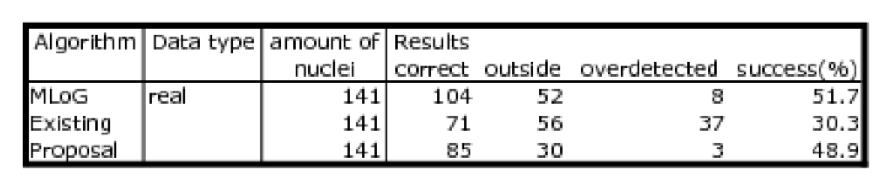
\includegraphics[width=1\textwidth]{pictures/evalReal}          
  \caption{Raw data from the evaluation framework. Processed data is a dataset from the ear of a zebrafish embryo.}
  \label{tab:realEvalRaw}
\end{figure}

This annex presents the raw results from the evaluation both on synthetic and real data of the existing algorithm in the Megason lab, the scale constrained Laplacien of Gaussian, and the proposed algorithm.
\section{Synthetic Data}
\begin{figure}[H]
  \centering
  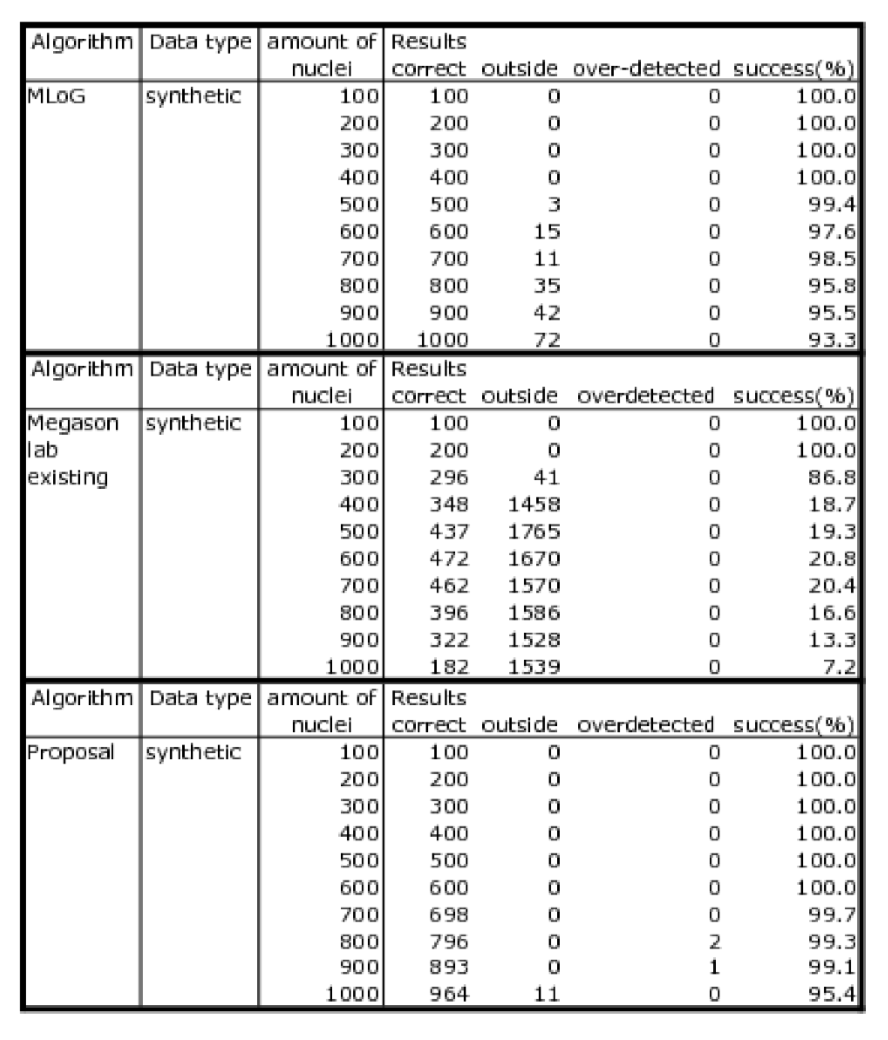
\includegraphics[width=1\textwidth]{pictures/evalTest}          
  \caption{Raw data from the evaluation framework. Processed data are 10 synthetic datasets with increaing number of nuclei and amount of noise.}
  \label{tab:syntheEvalRaw}
\end{figure}






%\input{ingenierie/AnnexesIngenierie}

\bibliographystyle{plain}
\bibliography{AntoBib}

\end{document}
